%! TeX program = lualatex
\documentclass[11pt]{report}
\usepackage{fontspec}
\newfontfamily\chapfont{Colonna MT}[Scale=2, Ligatures=TeX]
\newfontfamily\accentfont{CMU Serif}

\usepackage[
    sorting=nyt,
    style=verbose,
    backend=biber
]{biblatex}
\addbibresource{bibliography.bib}
\setlength\bibitemsep{2\itemsep}

\usepackage{import}

\usepackage{fancyhdr}
\pagestyle{fancy}
\fancyhf{}
\fancyfoot[C]{\thepage}
\setlength{\headheight}{2cm}
\renewcommand{\chaptermark}[1]{\markboth{\thechapter. \MakeUppercase{#1}}{}}
\renewcommand{\headrule}{}

\usepackage{titlesec}
\titleformat{\chapter}[display]
  {\chapfont\centering\Huge}{\thechapter}{15pt}{\LARGE}
\titlespacing*{\chapter}{0cm}{0cm}{15pt}

\titleformat{\section}
	{\sc}{\thesection}{1em}{\Large}

\titleformat{\subsection}
  {\sc}{\thesubsection}{1em}{\large}

\usepackage{tocloft}
\renewcommand{\contentsname}{\hfill\chapfont\LARGE Contents\hfill}
\renewcommand{\cftchappresnum}{\chapfont\Large}
\renewcommand{\cftchapfont}{\LARGE\sc}
\renewcommand{\cftsecfont}{\large\sc}
\renewcommand{\cftsubsecfont}{\sc}
\setcounter{tocdepth}{2}
\setlength{\cftbeforechapskip}{2\baselineskip}
\setlength{\cftbeforesecskip}{\baselineskip}
\setlength{\cftbeforesubsecskip}{0.75\baselineskip}
\setlength{\cftchapnumwidth}{1cm}

%Chapter outline env
\newenvironment{chout}{\begin{center}\it}{\end{center}}

\usepackage{xifthen}
\usepackage{pdfpages}
\usepackage{transparent}
\usepackage[nottoc]{tocbibind}

\usepackage{graphicx}
\graphicspath{ {./figures} }

\usepackage{xcolor}
\usepackage{float}
\usepackage{amsmath, amsfonts, amsthm, amssymb}
\usepackage[noabbrev]{cleveref}
\usepackage{enumerate}

% Figure related
\usepackage{tikz}
\usetikzlibrary{calc}
\usepackage{pgf}
\usepackage{caption}
\usepackage{subcaption}

% Page Geometry
\usepackage{geometry}
\geometry{a4paper, inner=2cm, outer=6.85cm, top=2cm, bottom=2cm, twoside,
marginparwidth=4.85cm}
\savegeometry{tufte}

\usepackage[framemethod=TikZ, innertopmargin=2mm, innerbottommargin=2mm,
innerleftmargin=2mm]{mdframed}

\usepackage{sidenotes}
\usepackage{mparhack}

% Theorems
\usepackage{thmtools}
\declaretheoremstyle[headfont=\sc, bodyfont=\normalfont, mdframed={
needspace=4\baselineskip, nobreak=false } ]{fullbox}
\declaretheoremstyle[headfont=\sc, bodyfont=\normalfont, mdframed={
rightline=false, topline=false, bottomline=false, needspace=4\baselineskip,
nobreak=false }]{sideline}

\declaretheorem[numberwithin=chapter, style=fullbox, name=Definition]{definition}
\declaretheorem[sibling=definition, style=fullbox, name=Theorem]{theorem}
\declaretheorem[sibling=definition, style=fullbox, name=Lemma]{lemma}
\declaretheorem[sibling=definition, style=fullbox, name=Corollary]{corollary}
\declaretheorem[sibling=definition, style=fullbox, name=Proposition]{proposition}
\declaretheorem[sibling=definition, style=sideline, name=Example]{example}
\declaretheorem[sibling=definition, style=sideline, name=Nonexample]{nonexample}
\declaretheorem[style=sideline, numbered=no, name=Remark]{remark}
\declaretheorem[style=sideline, numbered=no, name=Notation]{notation}

\setlength{\parskip}{0.3\baselineskip}
\setlength{\marginparpush}{0.5cm}
\setlength{\parindent}{0pt}

%Commands
\renewcommand{\vec}[1]{\textbf{#1}}
\renewcommand{\epsilon}{\varepsilon}
\newcommand{\defined}[1]{\textit{#1}\index{#1}}

%Operators
\DeclareMathOperator{\mult}{mult}
\DeclareMathOperator{\ord}{ord}
\DeclareMathOperator{\res}{Res}
\let\d\relax
\DeclareMathOperator{\d}{\, d\!}
\DeclareMathOperator{\im}{im}
\DeclareMathOperator{\coker}{coker}
\DeclareMathOperator{\supp}{supp}

%Indices
\usepackage{imakeidx}
\makeindex[columns=3, intoc, options = -s index.ist]

\author{Samuel Ireson}
\title{Riemann Surfaces}

\begin{document}
\pagenumbering{roman}
\newgeometry{inner=4cm, outer=4cm, top=2cm, bottom=2cm}
\begin{titlepage}
	\begin{center}
		\vspace{1cm}

		\LARGE\chapfont{Riemann surfaces}

		\vspace{1.0cm}

		% \normalsize\rm An analytic approach to Riemann surfaces, and the
		% Riemann-Roch theorem for compact Riemann surfaces.

		\vspace{0.5cm}

		\normalsize\sc{Samuel Ireson}

		\vfill

		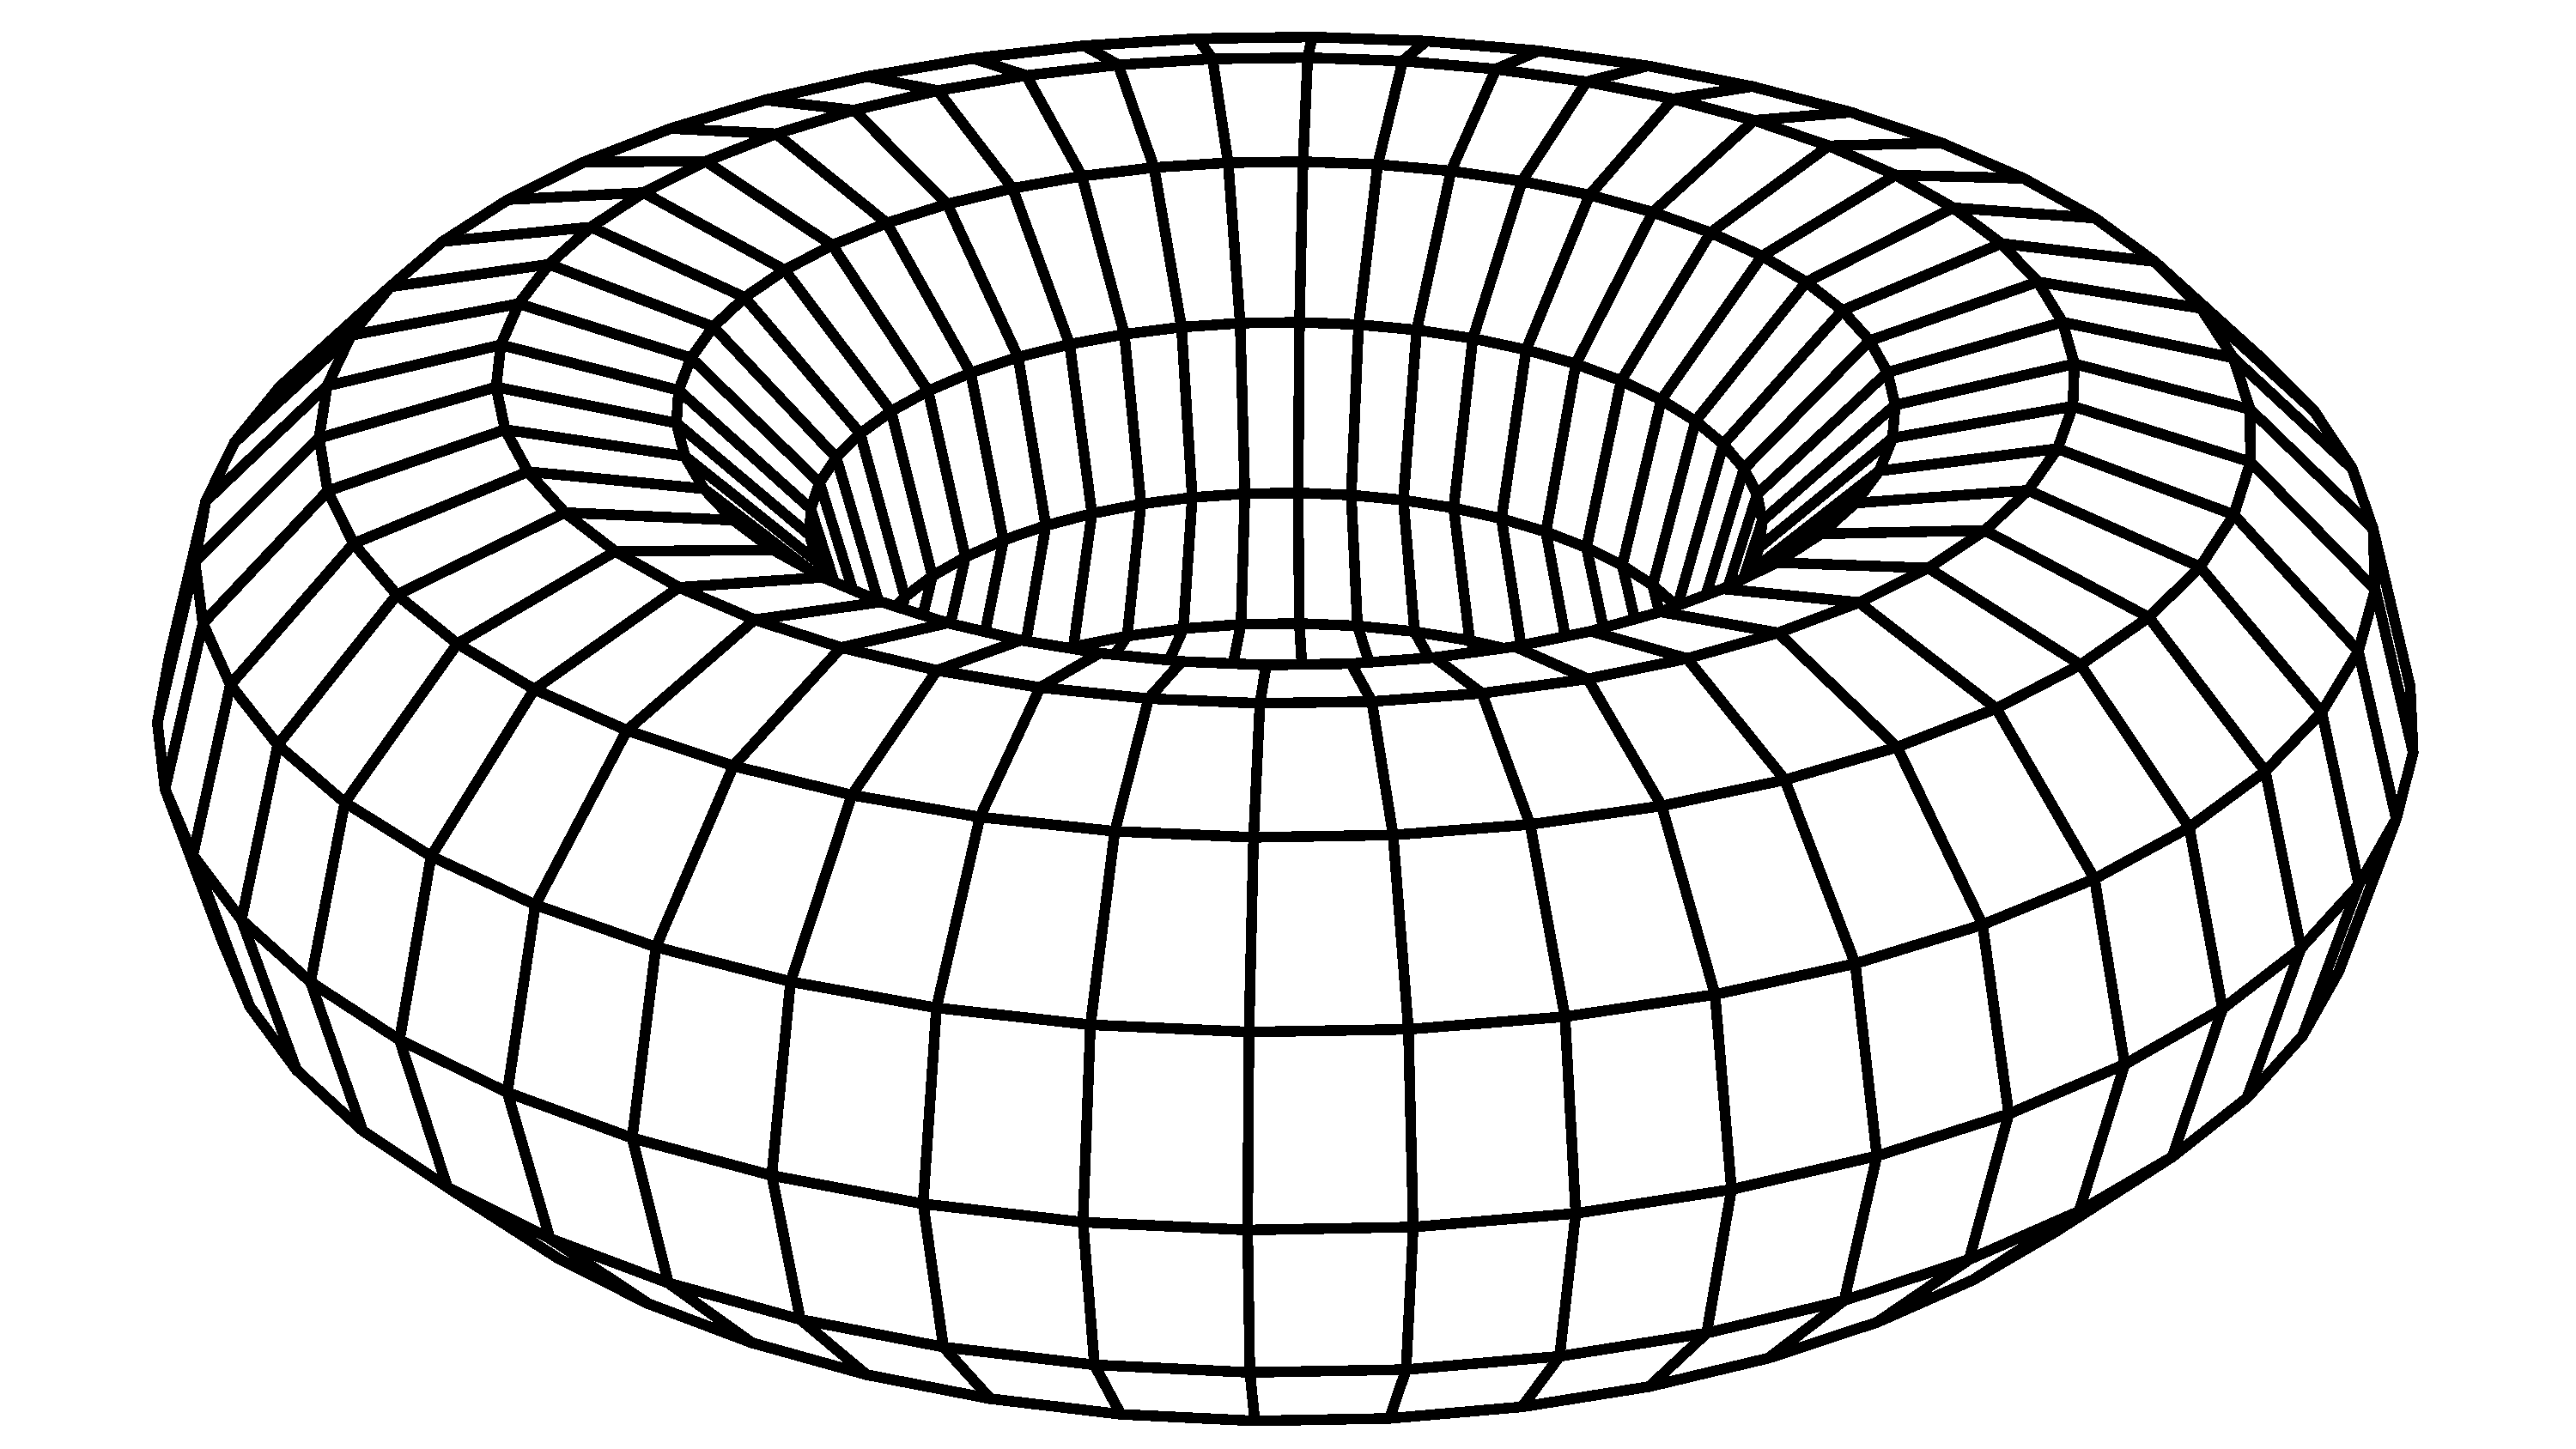
\includegraphics[width=\textwidth]{titlepage.pdf}

		\vfill

		Project III

		\vspace{0.5cm}

		Department of Mathematical Sciences

		\vspace{0.5cm}

		Durham University

	\end{center}

\end{titlepage}

\clearpage
\begin{center}
	% \thispagestyle{empty}
	\vspace*{\fill}
	For Mum,

	for Dad,

	{\accentfont за Девче}
	\vspace*{\fill}
\end{center}
\clearpage

% \thispagestyle{empty}
\vspace*{\fill}
This piece of work is a result of my own work and I have complied with the
Department's guidance on multiple submission and on the use of AI tools.
Material from the work of others not involved in the project has been
acknowledged, quotations and paraphrases suitably indicated, and all uses of AI
tools have been declared.
\vspace*{\fill}
\clearpage


\cleardoublepage
\tableofcontents
\restoregeometry

\pagenumbering{arabic}
\chapter*{Introduction}
First introduced in 1851, as part of Bernhard Riemann's doctoral
thesis\sidenote{\footnotesize\cite{riemann}}, Riemann surfaces have been central
to the development of mathematics in the 20$^{\mathrm{t h}} $ and 21$
	^{\mathrm{s t}} $ centuries. This publication sparked the rigorous and
methodical study of topology, and was responsible for drawing significant links
between complex analysis and algebraic geometry, an area essentially born of the
thesis. Riemann's discovery of these objects is representative of the
unification of many previously explored branches of theory, and this influence
is evident by the naming of key theorems throughout, for example with Abel's
addition theorem, and the Jacobi inversion theorem.

The first exploration of the concept, by Riemann himself, was concerned with
branches of multivalued complex functions, for example, the square root. Riemann
had the idea (``one of the most illuminating in the history of
mathematics''\sidenote{\footnotesize\cite{stillwell}}) to represent the relation
$ p ( x,y )=0 $ between $ x,y \in \mathbb{C} $ by covering a plane representing
the values of $ x $, by a surface representing the values of $ y $. We will
explore this idea and those related in Section~\ref{sec:affine-curves}.

\begin{figure}[h]
	\centering
	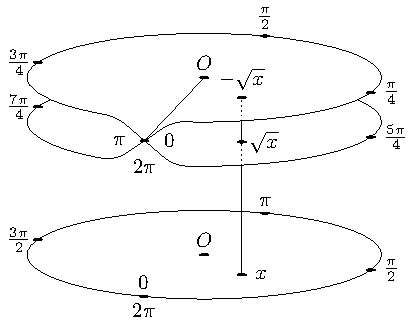
\includegraphics{sqrt-covering/figure}
	\caption{Freely deforming the unit disk such that the points $ y = \pm\sqrt{x}
		$ lie above $ x $.}
\end{figure}

The study of Riemann surfaces has behind it two remarkably distinct trails of
research and theory, paved respectively by complex manifold theory, and
algebraic geometry. We tend to explore the subject through the former
characterisation, but ommission of key results and ideas arising from the latter
would be misguided. As a result, there are chapters and sections of the report
which take more explicit notice of the algebraic geometric development, although
these are somewhat less integral to our main aim; the Riemann--Roch theorem for
compact Riemann surfaces.

\section*{Acknowledgement}
I am indebted to my project supervisor Raphael Zentner for his numerous resource
recommendations, for pushing me and my project in a direction both interesting
and challenging, and for the provision of herbal tea and chocolate.


\chapter{Preliminaries}\label{ch:prelims}
\begin{chout}
	The following chapter contains well-known definitions, and results from
	analysis and topology on which the content of this report will be built.
\end{chout}

\section{Topology}
Let $ X $ and $ Y $ be topological spaces.

\begin{definition}[Punctured neighbourhood]
	A \defined{punctured neighbourhood} $ P $ of $ x \in X $ is a set of the form
	$ P = Q \setminus \left\{ x \right\} $ where $ Q $ is an open neighbourhood of
	$ x $.
\end{definition}

\begin{definition}[Continuous map]
	A map $ f:X \to Y $ is called a \defined{continuous map} if $ f ^{-1}(V)
		\subseteq X $ is open for all open $ V \subseteq Y $.
\end{definition}

\begin{definition}[Open map]
	A map $ f:X \to Y $ is called an \defined{open map} if $ f(U)\subseteq Y $ is
	open for all open $ U \subseteq X $.
\end{definition}

\begin{definition}[Open cover]
	An \defined{open cover} of $ X $ is a collection $ (U_i)_{i \in I} $ of open
	subsets of $ X $ such that $ X = \bigcup_{i \in I}^{}{U_i} $.
\end{definition}

\begin{marginfigure}[-8cm]
	\centering
	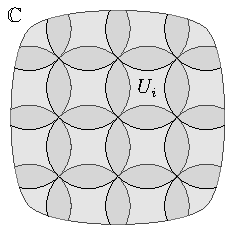
\includegraphics{open-cover/figure}
	\caption{The subsets $ U_{i} $ provide an open cover of $ \mathbb{C} $.}
\end{marginfigure}

\begin{definition}[Compactness]
	$ X $ is \defined{compact} if every open cover of $ X $ admits a finite
	subcover.
\end{definition}

\begin{marginfigure}[-4cm]
	\centering
	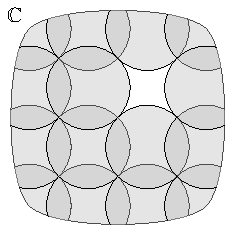
\includegraphics{compact/figure}
	\caption{This open cover does not admit a finite subcover, so $ \mathbb{C} $
		is non-compact.}
\end{marginfigure}
\vspace{-\baselineskip}

\section{Real Analysis}
Our work will primarily be in complex analysis, although preliminary
understanding of real analytic concepts will be useful. The following
definitions are due to Rudin\sidenote{\footnotesize\cite{rudin}}.

\begin{definition}[$ C ^{\infty} $]
	A real-valued function is $ C ^{\infty} $ if it has continuous derivatives to
	all orders on its domain. We sometimes refer to the set of $ C ^{\infty} $
	functions on domain $ X $ by $ C ^{\infty}(X;\mathbb{R}) $.
\end{definition}

\begin{definition}[Support]
	The \defined{support} of a function $ f $ on a topological space $ X $
	is the set
	\begin{align*}
		\supp f = \overline{\left\{ x \in X: f(x) \neq 0 \right\}}.
	\end{align*}
\end{definition}

\begin{definition}[Convolution]
	For two functions $ f,g: \mathbb{R}^{2}\to \mathbb{R} $, the
	\defined{convolution} of $ f $ and $ g $ is denoted and defined by
	\begin{align*}
		\left( f * g \right)(x) = \int_{\mathbb{R}^{2}}{f(y)g(x-y)}\d{y}.
	\end{align*}
\end{definition}

\begin{definition}[Cauchy sequence]
	Let $ H $ be an inner product space, and let $ \|\cdot\| = \left\langle \cdot
		, \cdot \right\rangle $ be the induced norm. A sequence $ \left( h_i \right)
		\in H $ is called a \defined{Cauchy sequence} if for every $ \epsilon>0 $
	there exists $ N \in \mathbb{N} $ such that
	\begin{align*}
		n,m \geq N \implies \|h_n - h_m\|<\epsilon.
	\end{align*}
\end{definition}

\begin{definition}[Hilbert space]
	A \defined{Hilbert space} $ \mathcal{H} $ is an inner product space which is
	\defined{complete}, i.e., a space in which every Cauchy sequence converges.
\end{definition}

\vspace{-0.8\baselineskip}
\section{Complex Analysis}
Let $ U \subseteq \mathbb{C} $ be open.

\begin{definition}[Holomorphicity]\label{def:holomorphicity}
	A function $ f:U \to \mathbb{C} $ is called \defined{holomorphic on} $ U'
		\subseteq U $ if it is complex differentiable at every point $ z \in U' $. The
	function is called \defined{holomorphic at} $ z_0 \in U $ if it is holomorphic
	on some open neighbourhood of $ z_0 $.
\end{definition}

\begin{definition}[Meromorphicity]
	A function $ f:U \to \mathbb{C} $ is called \defined{meromorphic at} $ z_0 \in U
	$ if it is holomorphic on a punctured neighbourhood of $ z_0 $, and has either a
	removable singularity, or pole at $ z_0 $.
\end{definition}

\vspace{-0.5\baselineskip}
We call $ D $ a \defined{domain} if it is an open, connected subset of $
	\mathbb{C} $. For the following two results, $ D $ is a domain, and $ f:D \to
	\mathbb{C} $ is holomorphic.

\begin{theorem}[Identity theorem]
	$ f $ is identically zero in $ D $ if the zero set of $ f $ has an
	accumulation/limit point in $ D $.
\end{theorem}

\begin{theorem}[Maximum modulus principle]\label{thm:pre-max-mod}
	If there exists a point $ z_0 \in D $ such that $ |f(z)|\leq|f(z_0)| $ for all
	points $ z \in D $, $ f $ is constant.
\end{theorem}

\vspace{-0.5\baselineskip}
We refer to holomorphic functions $ f:\mathbb{C} \to \mathbb{C} $ as
\defined{entire}, which allows us to state the following theorems succinctly.

\begin{theorem}[Open mapping theorem]
	A non-constant, entire map is open.
\end{theorem}

\begin{theorem}[Liouville's theorem]
	A bounded, entire map is constant.
\end{theorem}

\chapter{Manifold Theory}\label{ch:manifold-theory}
\begin{chout}
	The following chapter serves as an introduction to manifold theory which,
	through specification, will arrive us at the notion of a Riemann surface.
	The definitions are similar to those found in Lee\sidenotemark.
\end{chout}
\sidenotetext[][5\baselineskip]{\footnotesize\cite{lee}}

\section{Topological manifolds}
With an understanding of the direction in which our consideration is headed, we
introduce the following concepts in their complex version. There are times
however, when further intuition may be gained by consideration of the real
analogues of the definitions, and examples will be given when this is the case.
We start with a basic topological idea.

\begin{definition}[Hausdorff]
	A topological space $ X $ is \defined{Hausdorff} if for all distinct points $
		u,v \in X $ there exist open sets $ U \ni u $, $ V \ni v $ such that $ U \cap V
		= \varnothing $.
\end{definition}

\begin{marginfigure}
	\centering
	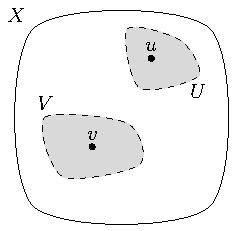
\includegraphics{hausdorff/figure}
	\caption{A Hausdorff space.}
\end{marginfigure}

\begin{example}\label{ex:complex-plane-discrete}
	Let $ \mathbb{C} $ have the discrete topology, that is, the topology with the
	basis of singleton sets in $ \mathbb{C} $. It is trivial that this space is
	Hausdorff; two distinct points $ z, \omega \in \mathbb{C} $ can be separated by
	their respective singletons, $ \left\{ z \right\} \cap \left\{ \omega \right\}
		= \varnothing $.
\end{example}

\begin{definition}[Locally Euclidean]
	Let $ X $ be a topological space. We say that $ X $ is \defined{locally
		Euclidean} of dimension $ n $, if for each $ x \in X $ there exists an open
	neighbourhood $ U_x $ of $ x $ homeomorphic, via homeomorphism $ \phi_x $, to an
	open subset $ \tilde{U}_{x}\subseteq \mathbb{C}^{n} $.
\end{definition}

\begin{marginfigure}[-3\baselineskip]
	\centering
	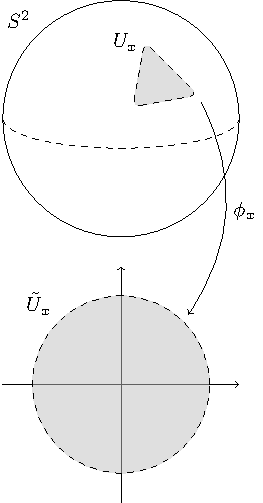
\includegraphics{s2-manifold/figure}
	\caption{$ S^2 $ is (real) locally Euclidean of dimension $ 2 $.}
\end{marginfigure}

\begin{remark}
	It is important to mention that reference to dimension will be implicit reference
	to \textit{complex} dimension, unless otherwise specified.
\end{remark}

The homeomorphisms, $ \phi_x $, are called \defined{coordinate functions}
(sometimes coordinates) at $ x $, motivated by the fact that they provide a
local Euclidean coordinate system on the space. Together with the domains on
which they are defined, coordinate functions are called \defined{charts},
denoted by $ (U_x, \phi_x) $. Any collection of chart domains which provides an
open cover of the space is called an \defined{atlas}, $ \{ U, \phi \} $.

\begin{example}[Complex plane with two
		origins]\label{ex:complex-plane-2-origins}
	Consider the space $ L $, constructed by taking two copies of $ \mathbb{C} $ and
	identifying all identical points apart from the origins. With greater formality,
	let
	\begin{gather*}
		L = \left( 0_a \times \mathbb{C} \sqcup 0_b \times \mathbb{C} \right)/{\sim}\\
		(0_a,z) \sim (0_b , z) \quad \forall z \in \mathbb{C}\setminus \left\{ 0 \right\}.
	\end{gather*}
	\begin{center}
		\begin{tikzpicture}
			\node (o) at (0,0){};
			\draw (-4,0) to (o);
			\draw (o) to (4,0) node[right]{$ \mathbb{C} $};
			\fill ($ (o) + (0,0.1) $) circle (0.05) node[above]{$ 0_a $};
			\fill ($ (o) - (0,0.1) $) circle (0.05) node[below]{$ 0_b $};
		\end{tikzpicture}
	\end{center}
	Describing the quotient topology on this space is straightforward; we can form a
	basis as follows. Firstly, we take the open sets of $ \mathbb{C}^{*} :=
		\mathbb{C}\setminus \left\{ 0 \right\} $, and join this collection with sets $
		(U \setminus \left\{ 0\right\}) \cup \left\{ 0_i \right\} $, for open $ U \subseteq
		\mathbb{C} $ containing $ 0 $.

	Since $ \mathbb{C}^{*} \subseteq \mathbb{C} $, we need only check if the two
	origin points $ 0_a $ and $ 0_b $ are locally Euclidean. The open neighbourhoods $
		\mathbb{C}_{i}:=\mathbb{C}^{*}\cup \left\{ 0_i \right\} $ of $ 0_i $ are both
	homeomorphic to $ \mathbb{C}$ via
	\begin{align*}
		\phi_i: \mathbb{C}_{i} \to \mathbb{C}: z \mapsto \begin{cases}
			                                                 z & z \in \mathbb{C}^{*} \\
			                                                 0 & z = 0_i
		                                                 \end{cases}
	\end{align*}
	and hence $ L $ is locally Euclidean of dimension $ 1 $.
\end{example}

Motivated in part by the existence of a few pathological counterexamples, the
definition of a topological manifold is often stated with the extra condition of
second-countability\sidenote{\footnotesize\cite[p. 36]{lee}}.

\begin{definition}[Second countability]
	A topological space $ X $ is called \defined{second countable} if it admits a
	countable basis for its topology.
\end{definition}

\begin{example}\label{ex:complex-cross}
	Let $ X = \left\{ (x,y) \in \mathbb{C}^{2}: xy=0 \right\} $. We aim to show that
	this set has a countable basis for the subset topology from $ \mathbb{C}^{2} $.
	Firstly, we note that $ \mathbb{R} $ admits a basis
	\begin{align*}
		\mathcal{B} = \left\{ (r,s) : r,s \in \mathbb{Q} \right\},
	\end{align*}
	i.e., the collection of open intervals in $ \mathbb{R} $ with rational
	endpoints. Further, $ \mathcal{B} $ has the same cardinality as $
		\mathbb{Q}^{2} = \mathbb{Q}\times \mathbb{Q} $ which is countable as the
	cartesian product of two countable sets (Figure~\ref{fig:Q-countable}). In
	particular, $ \mathbb{R} $ is second countable.

	$ \mathbb{R}^{4} $ is second countable when viewed as the fourth
	product of $ \mathbb{R} $ endowed with the product topology and since $
		\mathbb{R}^{4} \cong \mathbb{C}^{2} $, $ \mathbb{C}^{2} $ is also second
	countable. Finally, since second countability is hereditary, our claim is
	justified.
\end{example}

\begin{marginfigure}[-15\baselineskip]
	\centering
	\resizebox{\columnwidth}{!}{
		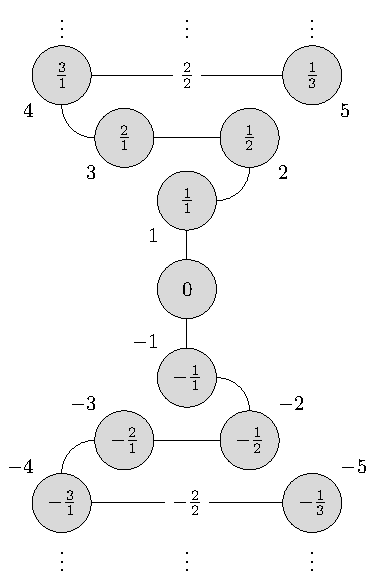
\includegraphics{Q-countable/figure}
	}
	\caption{$ \mathbb{Q} $ is countable.}
	\label{fig:Q-countable}
\end{marginfigure}

It is interesting to note that a restriction to topological spaces with
countable topologies is too heavy-handed. We would like to be able to consider
$ \mathbb{C} $ as a manifold, but even this space has uncountably many open
sets.

\begin{definition}[Topological manifold]
	An $ n $-dimensional \defined{topological manifold} is a second-countable,
	Hausdorff space, which is locally Euclidean of dimension $ n $.
\end{definition}

\begin{nonexample}
	Example~\ref{ex:complex-cross} is not locally Euclidean.

	Example~\ref{ex:complex-plane-2-origins} is not Hausdorff.

	Example~\ref{ex:complex-plane-discrete} is not second countable.
\end{nonexample}

\begin{example}\label{ex:C-top-manifold}
	Trivial examples of topological manifolds are $ \mathbb{C}^{n} $ with the
	standard topology, and subsets $ U \subseteq \mathbb{C}^{n} $ with the induced
	subset topology. The identity map over the whole space provides a suitable atlas
	in both cases.
\end{example}

Before examining further non-trivial examples in detail, we consider the
imposition of further structure on a manifold, as this leads the way to more
interesting results.

\section{Complex analytic manifolds}
Further restrictions on manifolds are imposed via the charts which define them.

\begin{definition}[Compatible charts]
	The charts $ (U_x, \phi_x) $ and $ (U_y, \phi_y) $ on a topological space $ X $
	are said to be \defined{compatible} if
	\begin{align*}
		\phi _{x,y}:= \phi_x \circ \phi_y ^{-1}: \phi_y(U_x \cap U_y) \to \phi_x(U_x
		\cap U_y)
	\end{align*}
	is holomorphic. Charts are \defined{vacuously compatible} if $ U_{x}\cap
		U_{y}\neq\varnothing $.
\end{definition}

\begin{figure*}
	\centering
	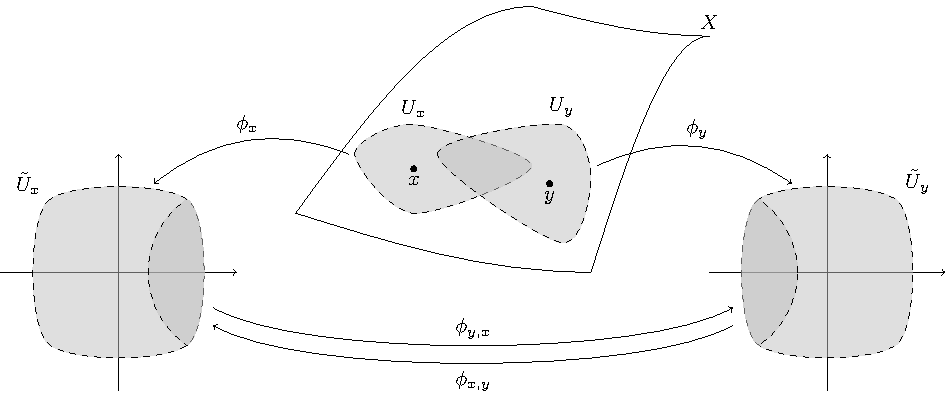
\includegraphics{transition-fcts/figure}
	\caption{We call the functions $ \phi _{x,y} $ and $ \phi _{y,x} $ \defined{transition
			functions}.}
\end{figure*}

\begin{remark}
	From initial inspection it is clear that this definition is
	symmetric\sidenotemark. If $ \phi _{x,y}$ is holomorphic on $ \phi_y(U_x \cap
		U_y) $ then $ \phi _{y,x} $ will also be holomorphic on $ \phi_x(U_x \cap U_y)
	$. Reflexivity of the relation is also clear, as a result of the holomorphicity
	of the identity function.

	We cannot \textit{a priori} make an analogous statement on the transitivity of
	this relation. Suppose that $ (U_1, \phi_1) $ is compatible with $ (U_2, \phi_2)
	$ which is in turn compatible with $ (U_3, \phi_3) $. The composition
	\begin{align*}
		\phi_3 \circ \phi_1 ^{-1} = \left( \phi_3 \circ \phi_2 ^{-1} \right) \circ
		\left( \phi_2 \circ \phi_1 ^{-1} \right)
	\end{align*}
	is holomorphic on the domain $ \phi_1(U_1 \cap U_2 \cap U_3) $ but not
	necessarily $ \phi_1(U_1 \cap U_3) $.
\end{remark}
\sidenotetext[][-12\baselineskip]{\footnotesize\cite[p. 2]{miranda}}

\begin{definition}[Complex analytic manifold]
	A manifold is \defined{analytic} if it has pairwise compatible coordinate charts.
\end{definition}

\begin{remark}
	It is interesting at this point\sidenotemark\ to consider the different
	structures which we could have imposed on a manifold.
	\begin{itemize}
		\item If we decided that our transition functions should be differentiable, we
		      would arrive at the definition of a differentiable manifold.
		\item If we asserted that the transition functions should be $ C ^{\infty} $,
		      we would recover the notion of a smooth manifold.
		\item If we required the transition functions to be $ C ^{\infty} $ with
		      positive Jacobian, we would consider oriented smooth manifolds.
	\end{itemize}
	all of which have interesting associated theory and applications.
\end{remark}
\sidenotetext[][-15\baselineskip]{\footnotesize\cite[p. 30]{donaldson}}

We will now consider the Riemann sphere $ \hat{\mathbb{C}} $, which we define
via Alexandroff's\sidenote{\footnotesize\cite{alexandroff}} one-point
compactification to be
\begin{align*}
	\hat{\mathbb{C}} = \mathbb{C} \cup \left\{ \infty \right\}.
\end{align*}

\begin{marginfigure}[-15\baselineskip]
	\centering
	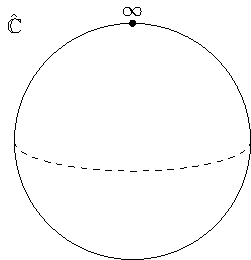
\includegraphics{Chat/figure}
	\caption{$ \hat{\mathbb{C}}\cong S^2$}
\end{marginfigure}

We take the topology of $ \hat{\mathbb{C}} $ to be the collection of open sets
in $ \mathbb{C} $ together with unions $ \left\{ \infty \right\}\cup \left(
	\mathbb{C}\setminus K \right) $ for compact $ K \subseteq \mathbb{C}$.

\begin{marginfigure}
	\centering
	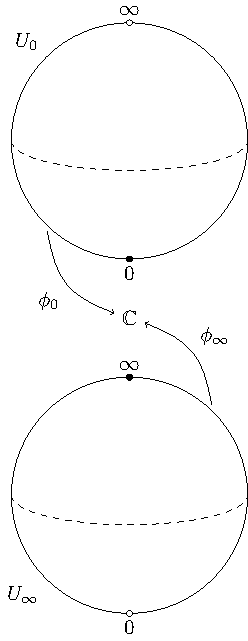
\includegraphics{Chat-analytic-manifold/figure}
	\caption{$ \hat{\mathbb{C}} = U_0 \cup U _{\infty} $}
\end{marginfigure}

\begin{example}\label{ex:Ch-analytic-manifold}
	We now aim to impose the structure of a complex analytic manifold on the Riemann
	sphere. To begin, consider the following subsets of $ \hat{\mathbb{C}} $,
	\begin{gather*}
		U_0 = \hat{\mathbb{C}}\setminus \left\{ \infty \right\} = \mathbb{C},\\
		U_{\infty} = \hat{\mathbb{C}} \setminus \left\{ 0 \right\}.
	\end{gather*}
	We note that $ U_0 \cup U _{\infty} = \hat{\mathbb{C}} $ and furthermore, $ U_0
		\cap U _{\infty} = \mathbb{C}^{*} $. Both of these subsets are homeomorphic to
	$ \mathbb{C} $ via the coordinate functions,
	\begin{gather*}
		\phi_0:U_0 \to \mathbb{C}:z \mapsto z,\\
		\phi _{\infty}:U _{\infty}\to \mathbb{C}:z \mapsto \begin{cases}
			\frac{1}{z} & z \in \mathbb{C}, \\
			0           & z = \infty.
		\end{cases}
	\end{gather*}
	It remains to verify that the transition functions are holomorphic, in
	particular, holomorphic on $ \mathbb{C}^{*} $. The transition functions are
	given by,
	\begin{align*}
		\phi _{0, \infty} = \phi_0 \circ \phi _{\infty}^{-1} = \frac{1}{z} = \phi
		_{\infty} \circ \phi_0 ^{-1} = \phi _{\infty, 0}.
	\end{align*}
	Clearly, $ z \mapsto 1/z $ is holomorphic on $ \mathbb{C}^{*} $, and hence $
		\left\{ (U_0, \phi_0), (U _{\infty}, \phi _{\infty}) \right\} $ is a suitable atlas.
\end{example}

It is reasonable at this point to ask whether this is the only possible atlas by
which the Riemann sphere is seen to be a complex analytic manifold. Under our
current understanding of the definition, this is clearly not the case. We may
trivially add charts to this atlas which are contained by the current charts,
without fundamentally changing the structure of the manifold. We would like for
manifolds obtained in this manner to be considered equivalent.

\begin{definition}[Compatible atlases]
	Two atlases $ \mathcal{A} $ and $ \mathcal{B} $ are said to be
	\defined{compatible} if $ \mathcal{A}\cup \mathcal{B} $ is an atlas.
\end{definition}

We note that this condition essentially makes a statement about the
compatibility of the charts in each of the atlases. In particular, every chart
in $ \mathcal{A} $ is compatible with every chart in $ \mathcal{B} $. In this
case, we often say that the charts of $ \mathcal{A} $ are compatible with $
	\mathcal{B} $.

\begin{lemma}\label{lem:compatibility-transitivity}
	If two charts are individually compatible with the atlas $ \mathcal{A} $, they
	are compatible with eachother.
	\begin{proof}
		Let $ \left\{ U _{\alpha}, \phi _{\alpha} \right\} $ be an atlas for the
		manifold $ M $, and consider two additional charts on $ M $, $ (V, \varphi) $
		and $ (W, \gamma) $ compatible with this atlas. If $ V \cap W = \varnothing
		$, we are done, and we hence make the contrary assumption. Let $ m \in V
			\cap W $. Since $ m \in M $, there exists some chart, say $ (U_m, \phi_m) $,
		such that $ m \in U_m $. Therefore, $ m \in V \cap W \cap U_m $.

		We remarked on the transitivity of compatibility on the intersection of three
		chart domains, and by this remark the transition function $ \varphi \circ \gamma
			^{-1} $ is holomorphic on $ \gamma(V \cap W \cap U_m) $. Specifically, it is
		holomorphic at the point $ \gamma(m) $, and the initially arbitrary choice of $
			m $ determines that the transition function is holomorphic on $ \gamma(V \cap W)
		$.
	\end{proof}
\end{lemma}

\begin{marginfigure}[-15\baselineskip]
	\centering
	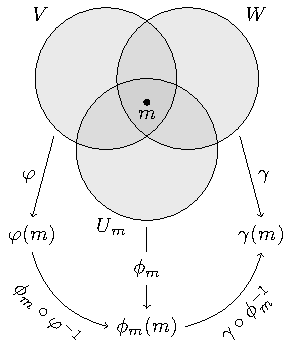
\includegraphics{atlas-compatibility/figure}
	\caption{The composition of two holomorphic functions $ \gamma \circ \phi_m
			^{-1} $ and $ \phi_m \circ \varphi ^{-1} $.}
\end{marginfigure}

An atlas $ \mathcal{M} $ is said to be \defined{maximal} if it cannot be
contained by any other atlas. The following result allows us to define the
notion of equivalence of analytic manifolds.

\begin{proposition}
	Every atlas $ \mathcal{A} $ is contained in a unique maximal atlas $ \mathcal{M}
	$.
	\begin{proof}
		Let $ \mathcal{C} $ denote the set of charts compatible with the atlas $
			\mathcal{A} $, and let $ \mathcal{M} = \mathcal{A}\cup \mathcal{C} $. The charts
		in $ \mathcal{C} $ are pairwise compatible by
		Lemma~\ref{lem:compatibility-transitivity} and hence $ \mathcal{M} $ is an
		atlas. This atlas is maximal since any chart compatible with $ \mathcal{M} $ is
		compatible with the sub-atlas $ \mathcal{A} $ and is hence contained by $
			\mathcal{M} $.

		To see that this atlas is unique, let $ \mathcal{M}' $ denote another maximal
		atlas containing $ \mathcal{A} $. Every chart in $ \mathcal{M}' $ is compatible
		with $ \mathcal{A} $ and hence the method of construction of $ \mathcal{M} $
		determines that $ \mathcal{M}' \subseteq \mathcal{M} $. Since both atlases are
		maximal, it must be the case that $ \mathcal{M}'=\mathcal{M} $.
	\end{proof}
\end{proposition}

As a final\'e to the chapter, we introduce the definition of equivalence of
manifolds. We could have, and it is often seen in the
literature\sidenote{\footnotesize\cite{miranda}}, included this notion of
equivalence directly in the definition of the manifold.

\begin{definition}[Equivalent manifolds]
	Let $ X $ and $ Y $ be two complex analytic manifolds, with respective atlases,
	$ \mathcal{X} $ and $ \mathcal{Y} $. $ X $ and $ Y $ are said to be
	\defined{equivalent} if $ \mathcal{X} $ and $ \mathcal{Y} $ are contained in the
	same maximal atlas.
\end{definition}

As our study progresses, we will see an alternative formulation of equivalence,
which is somewhat more intuitive and follows more readily from complex analysis.
The formulation presented is however the standard in modern manifold theory, and
is therefore useful for future consideration.

\chapter{Riemann Surfaces}
\begin{chout}
	We now define Riemann surfaces, considering initial examples.
\end{chout}

\section{Definition}
\begin{definition}[Riemann surface]
	A \defined{Riemann surface} is a connected, one-dimensional complex analytic
	manifold.
\end{definition}

\begin{remark}
	Since we made the inclusion of second countability in our definition of a
	topological manifold, it is important to make comment on the fact that this
	inclusion is redundant for Riemann surfaces. In particular, every connected
	Riemann Surface is second countable; a highly non-trivial result due to Tibor
	Rad\'o\sidenotemark.

	We also note that an assertion of connectedness is not universal in the
	literature, but for our considerations, it is convenient.
\end{remark}
\sidenotetext[][-4\baselineskip]{\footnotesize \cite{rado}}

The concision of this definition is maybe unexpected, and it is
common\sidenote{\footnotesize\cite[p. 29]{donaldson}} to define Riemann surfaces
with a more verbose definition without the abstraction to manifolds, although
our approach is equivalent. A keen eye will note that this definition also
determines that we have already encountered an example of a Riemann surface ---
the Riemann sphere $ \hat{\mathbb{C}} $, is one dimensional and a suitable atlas
was given in Example~\ref{ex:Ch-analytic-manifold}.

\begin{example}\label{ex:C-open-subset}
	With reference to Example~\ref{ex:C-top-manifold}, $ \mathbb{C} $ is a Riemann
	surface. We call this Riemann surface the \defined{complex plane}.
\end{example}

We now consider some further examples in full detail as these will be useful in
providing future examples as we develop the theory in parallel.

\section{Projective line}
\begin{definition}[Complex Projective Line]
	The \defined{complex projective line}, denoted $ \mathbb{C}\mathbb{P}^{1} $ is
	the set of one dimensional subspaces of $ \mathbb{C}^{2} $.
\end{definition}

\begin{marginfigure}[-3\baselineskip]
	\centering
	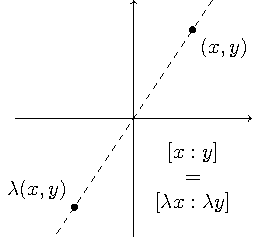
\includegraphics{real-projective/figure}
	\caption{It is useful to consider these notions via their real analogues.}
\end{marginfigure}

We know from linear algebra that one dimensional subspaces are spanned by a
single element. For an element $ (x,y) \in \mathbb{C}^{2}\setminus \left\{ 0
	\right\} $, we denote the span of $ (x,y) $ by,
\begin{align*}
	[x:y] = \left\{ \lambda(x,y): \lambda \in \mathbb{C} \right\}.
\end{align*}
Hence, an alternative expression of $ \mathbb{C}\mathbb{P}^{1} $ is given as,
\begin{align*}
	\mathbb{C}\mathbb{P}^{1} = \left\{ [x:y]:(x,y) \in \mathbb{C}^{2}\setminus
	\left\{ 0 \right\} \right\}.
\end{align*}
We refer to the elements $ [x:y] \in \mathbb{C}\mathbb{P}^{1} $ as
\defined{homogeneous coordinates} since $ \forall \lambda \in
	\mathbb{C}^{*} $,
\begin{align*}
	[x:y] = [\lambda x: \lambda y].
\end{align*}

We now aim to give topological structure to $ \mathbb{C}\mathbb{P}^{1} $, and
from this, Riemann surface structure. For this process, we take inspiration from
Miranda\sidenote{\footnotesize\cite[p. 8]{miranda}}.

Consider the following two subsets of $ \mathbb{C}\mathbb{P}^{1} $,
\begin{align*}
	U_x & = \left\{ [x:y] : x \neq 0 \right\}, \\
	U_y & = \left\{ [x:y] : y \neq 0 \right\},
\end{align*}
which are clearly such that $ \mathbb{C}\mathbb{P}^{1} = U_x \cup U_y $. We
consider the following functions on these subsets;
\begin{align*}
	\phi_x: U_x \to \mathbb{C}: [x:y] \mapsto \frac{y}{x}, \\
	\phi_y: U_y \to \mathbb{C}: [x:y] \mapsto \frac{x}{y}.
\end{align*}
It is clear that these functions are respectively bijective. With this we can
give each $ U_i $ a topology; a set $ U \subseteq U_i $ is open if and only if $
	\phi_i(U) $ is open in $ \mathbb{C} $. Since the subsets $ U_i $ cover $
	\mathbb{C}\mathbb{P}^{1} $ we can equally well give this space a topology,
asserting that $ U \subseteq \mathbb{C}\mathbb{P}^{1} $ is open if and only if $
	U \cap U_i $ is open for each $ i=x,y $.

This definitively determines that $ (U_x, \phi_x) $ and $ (U_y, \phi_y) $
are charts on $ \mathbb{C}\mathbb{P}^{1} $, and furthermore, these charts are
compatible, since
\begin{align*}
	\phi_x \circ \phi_y ^{-1}(z) = \frac{1}{z} = \phi_y \circ \phi_x ^{-1}(z)
\end{align*}
is holomorphic on $ \phi_x(U_x \cap U_y) = \mathbb{C}^{*} = \phi_y(U_x \cap U_y)
$.

It remains to show that $ \mathbb{C}\mathbb{P}^{1} $ is Hausdorff. As usual,
we consider two points $ p,q \in \mathbb{C}\mathbb{P}^{1} $. If these points are
simultaneously contained by either $ U_x $ or $ U_y $, they may be separated by
disjoint open sets since the $ U_i $ are individually Hausdorff. The remaining
case is that of the points $ p=[1:0] $ and $ q=[0:1] $. These points are
respectively contained by the disjoint sets $ \phi_x ^{-1}(D) $ and $ \phi_y
	^{-1}(D) $ where $ D \subseteq \mathbb{C} $ is the open unit
disc\sidenote{\footnotesize\cite[p. 9]{miranda}}.

\begin{remark}
	There is a remarkable similarity between the approach seen here and the one we
	took for the Riemann sphere, which is, as usual in mathematics, no
	coincidence. We can show that as topological spaces $ \hat{\mathbb{C}} $ and $
		\mathbb{C}\mathbb{P}^{1} $ are homeomorphic via the map
	\begin{align*}
		g: \hat{\mathbb{C}} \to \mathbb{C}\mathbb{P}^{1}:z \mapsto \begin{cases}
			                                                           [z:1] & z \neq \infty \\
			                                                           [1:0] & z = \infty
		                                                           \end{cases}
	\end{align*}
	which is continuous and has continuous inverse,
	\begin{align*}
		h: \mathbb{C}\mathbb{P}^{1} \to \hat{\mathbb{C}}: [x:y] \mapsto \begin{cases}
			                                                                \frac{x}{y} & y \neq0 \\
			                                                                \infty
			                                                                            & y = 0.
		                                                                \end{cases}
	\end{align*}
	Furthermore, we will see in Section~\ref{sec:riemann-roch} that there is only
	one possible holomorphic structure on $ \hat{\mathbb{C}} $, the same as the
	one we have given to $ \mathbb{C}\mathbb{P}^{1} $.
\end{remark}

\section{Complex Tori}\label{sec:complex-tori}
We now aim to give Riemann surface structure to complex tori. We will, in fact,
consider one specific torus, although the approach is easily generalisable.
Firstly, we recall the definition of the Gaussian integers,
\begin{align*}
	\mathbb{Z} \oplus i \mathbb{Z} = \left\{ a + ib: a,b \in \mathbb{Z} \right\}
\end{align*}
which we choose to refer to by $ \Lambda $.

\begin{marginfigure}
	\centering
	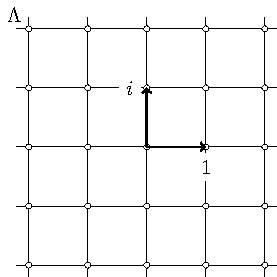
\includegraphics{lattice/figure}
	\caption{We refer to discrete additive subgroups like $ \Lambda $ as lattices.}
\end{marginfigure}

We can construct the quotient space $ \mathbb{C}/\Lambda $, which is more
explicitly expressed as,
\begin{gather*}
	\mathbb{C}/{\sim} = \left\{ [z]: z \in \mathbb{C} \right\},\\
	[z] = \left\{ \omega \in \mathbb{C}: z \sim \omega \right\},\\
	z\sim \omega \iff z-\omega \in \Lambda.
\end{gather*}

This space has a natural quotient topology via the projection map $
	\pi:\mathbb{C}\to \mathbb{C}/\Lambda: z \mapsto [z] $. Further to this, we can
show that $ \pi $ is open --- considering an open set $ U \subseteq \mathbb{C}
$, showing that $ \pi(U) $ is open is simply noticing that
\begin{align*}
	\pi ^{-1}(\pi(U)) = \bigcup_{\lambda \in \Lambda}^{}{(\lambda + U)}
\end{align*}
is a union of translations of $ U $ by elements in $ \Lambda $; hence open.

\begin{marginfigure}
	\centering
	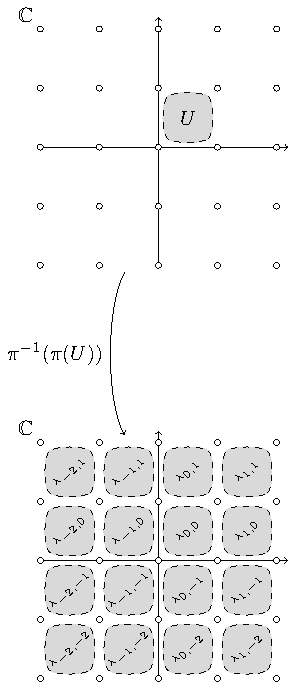
\includegraphics{pi-open/figure}
	\caption{$ \lambda _{a,b} = U + a + ib $}
\end{marginfigure}

In order to find a covering set of charts, we consider sets of the form
\begin{align*}
	B(z_0;\epsilon) = \left\{ \omega \in \mathbb{C}: |z_0-z|<\epsilon \right\},
\end{align*}
and note that for $ 0<\epsilon<\frac{1}{2} $, the map $
	\pi|_{B(z_0;\epsilon)}:B(z_0;\epsilon) \to \pi(B(z_0;\epsilon))$ is injective.
Furthermore, as a restriction of $ \pi $, this map is continuous, surjective,
and open, and this is sufficient to state $ \pi|_{B(z_0;\epsilon)} $ as a
homeomorphism between these two sets. Setting $ \phi _{z_0} $ to be the inverse of
this homeomorphism gives us a complex chart at the point $ \pi(z_0) = [z_0] $.
This shows $ \mathbb{C}/\Lambda $ to be locally Euclidean, and the compatibility
of these charts is all that stands between the realisation of a Riemann surface
structure.

For brevity, let $ U _{\alpha} $ denote the domain of the coordinate $ \phi
	_{\alpha} $, that is, the set $ \pi(B(\alpha; \epsilon)) $. The transition
function $ \phi _{z, \omega}: \phi _{\omega}(U_z \cap U _{\omega}) \to \phi
	_{z}( U_z \cap U _{\omega}) $ is such that
\begin{align*}
	\pi(\phi _{z,\omega})(u) & = \pi( \phi_z \circ \phi_{\omega}^{-1})(u) \\
	                         & = \phi_{\omega}^{-1}(u)                    \\
	                         & = \pi(u)
\end{align*}
for every $ u \in \phi _{\omega}(U_z \cap U _{\omega}) $, and notably, this
determines that $ \phi _{\omega}(u) \sim u $. We now observe that $ \phi _{z,
		\omega} $ is continuous, and that $ \Lambda $ is discrete. $ \phi _{z,
		\omega}(u)-u $ is therefore constant on the connected components of $ \phi
	_{\omega}(U_z \cap U _{\omega}) $ and $ \phi _{z, \omega} $ is holomorphic. The
charts are compatible.

To justify our naming of the section as `Complex Tori' we claim that the above
constructed quotient space is homeomorphic to the torus, defined as $ S^1 \times
	S^1$ for $ S^1 = \left\{ z \in \mathbb{C}: |z|=1 \right\} $. Finding an
explicit homeomorphism is not difficult, and we do this now. Consider the point
$ [z_0] \in \mathbb{C}/\Lambda $ and let one of the representatives of this
point be given as $ z_0 = a + ib $ for $ a,b \in \mathbb{R} $. Then, the map
\begin{align*}
	f & : \mathbb{C}/\Lambda \to S^1 \times S^1                       \\
	  & : [z_0] \mapsto \left( e ^{2 a\pi i}, e ^{2 b \pi i} \right).
\end{align*}
is a homeomorphism. The well-definedness of this map is seen by considering the
periodicity of each of the coordinates in the image, and the other conditions
for a homeomorphism follow easily from properties of the exponential function.
We can get better intuition for this homeomorphism if we think about the set $
	P_0 = \left\{ z \in \mathbb{C}: 0 \leq \mathfrak{Im}(z) < 1, 0 \leq
	\mathfrak{Re}(z) < 1\right\} $. Each point in $ \mathbb{C}/\Lambda $ has a
unique representative in this set, and furthermore, the closure of the set, has
double representatives only on its boundary. Identifying these points in the way
described by the equivalence relation gives us the following mental picture.

\begin{figure*}
	\centering
	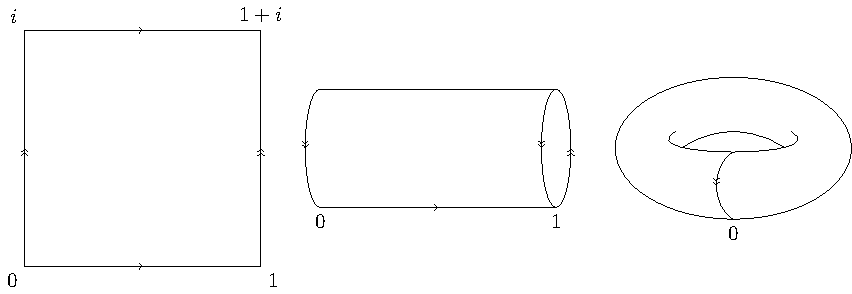
\includegraphics{torus-id/figure}
	\caption{The intuition behind the homeomorphism.}
\end{figure*}

Statement can then be made on the topological properties of the Riemann surface
we constructed; $ \mathbb{C}/\Lambda $ is a compact Riemann surface of genus
one.

\section{Affine curves}\label{sec:affine-curves}
\begin{definition}[Affine curve]
	An \defined{affine curve} is the zero locus of a polynomial $ f(x,y) $ in $
		\mathbb{C}^{2} $,
	\begin{align*}
		X = \left\{ (x,y) \in \mathbb{C}^{2}: f(x,y)=0 \right\}.
	\end{align*}
\end{definition}

\begin{marginfigure}
	\centering
	\resizebox{\columnwidth}{!}{
		\import{figures/affine-curve}{trifolium.pgf}
	}
	\resizebox{\columnwidth}{!}{
		\import{figures/affine-curve}{lemniscate.pgf}
	}
	\caption{The trifolium, and lemniscate, two real affine curves.}
\end{marginfigure}


The following section is concerned with giving Riemann surface structure to
affine curves which have a certain property; smoothness.

\begin{definition}[Smooth affine curve]
	An affine curve $ X $ defined by polynomial $ f(x,y) \in \mathbb{C}[x,y] $
	is called smooth if at all points $ x \in X $, \begin{align*}
		\frac{\partial f}{\partial x} \neq 0 \quad \text{ or } \quad \frac{\partial
			f}{\partial y}\neq 0.
	\end{align*}
\end{definition}

We introduce this restriction for good reason. The Implicit Function
Theorem\sidenote{\footnotesize\cite[p. 10]{miranda}}, tells us that under this
restriction, there always exists a function $ g $ such that the affine curve is
locally the graph of $ g $. This is particularly useful since it allows us to
give Riemann surface structure to these curves.

Suppose that $ X $ is a smooth affine curve; the zero locus of a polynomial $
	f(x,y) $, and take a point $ p \in X $. If $ \partial f/\partial x(p)
	\neq 0 $, we can take the projection map $ \pi_x:(x,y) \mapsto x $ to be a
complex chart in a neighbourhood of the point $ p $, which has a continuous
inverse $ \pi_x ^{-1}:x \mapsto (x,g_p(x)) $ where $ g_p $ is the function which
exists by the Implicit Function Theorem. Alternatively, if $ \partial f/\partial
	x(p)=0 $, the smoothness of $ X $ forces that $ \partial f/\partial y(p)\neq0
$ and we can make an identical construction.

\begin{marginfigure}
	\centering
	\resizebox{\columnwidth}{!}{
		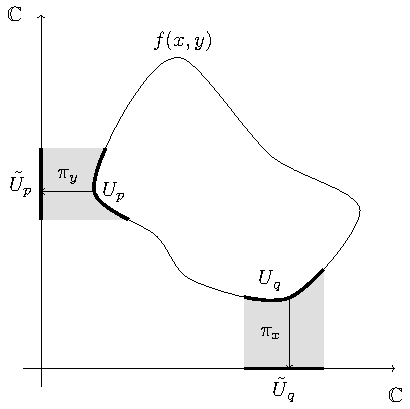
\includegraphics{implicit-fct-thm/figure}
	}
	\caption{Finding charts on smooth affine curves.}
\end{marginfigure}


Of course, we still need to check that these charts are compatible, and there
are two main cases to consider. Let $ U_p $ and $ U_q $ be neighbourhoods of two
points $ p,q \in X $. If the coordinate functions defined on both of these domains, are the
first projection, that is $ \pi_x $, the transition function is nothing more
than the identity, which is holomorphic. If, without loss of generality, the
coordinate function on $ U_p $ is $ \pi_x $ and on $ U_q $, $ \pi_y $, the
transition function, has the action
\begin{align*}
	\pi _{x,y} = \pi_x \circ \pi_y ^{-1}: y \mapsto (y,g(y)) \mapsto g(y),
\end{align*}
where $ g(y) $ is the holomorphic local representation of $ f(x,y) $ whose
existence is assured by the Implicit Function Theorem.

The second countability and Hausdorffness of $ X $ follow hereditarily from $
	\mathbb{C}^{2} $, and if we assert that the function $ f $ is irreducible,
then $ X $ is also connected\sidenote{\footnotesize\cite[p. 127]{shafarevich}}.

\begin{remark}
	We note that smooth affine curves give us our first non-trivial example of
	non-compact Riemann surfaces --- the Heine--Borel theorem states that compact
	subsets of $ \mathbb{C}^{2} $ must be bounded, but for all $ x_{0}\in
		\mathbb{C} $, there exists $ y \in \mathbb{C} $ such that $ f ( x_{0},y )=0
	$.
\end{remark}

\section{Projective curves}\label{sec:projective-curves}
The previous remark gives motivation for this section on projective curves. In
the same way that the compactification of the complex plane arrived us at the
Riemann sphere, compactification of algebraic curves will arrive us at a
collection of examples central to the theory of compact Riemann surfaces.

\begin{definition}[Complex Projective Space]
	Let $ u,v \in \mathbb{C}^{n} $, and let $ u \sim v \iff \exists \lambda \in
		\mathbb{C}^{*} $ such that $ u= \lambda v $. \defined{Complex projective
		space}, denoted by $ \mathbb{C}\mathbb{P}^{n} $ is defined as,
	\begin{align*}
		\mathbb{C}\mathbb{P}^{n} = \mathbb{C} ^{n+1}/{\sim},
	\end{align*}
	i.e., the quotient space of $ \mathbb{C}^{n+1} $ by the multiplicative action
	of $ \mathbb{C}^{*} $.
\end{definition}

It is easy to see that for $ n=1 $, this definition coincides with our original
definition for the complex projective line. This alternative formulation is
useful since it makes the Hausdorff nature of the space more overtly obvious ---
the quotient topology from the natural projection map will be Hausdorff. Complex
projective space has other desirable features, such as compactness.

\begin{proposition}
	$ \mathbb{C}\mathbb{P}^{n} $ is compact.
	\begin{proof}
		Let $ \pi: \mathbb{C}^{n}\setminus \left\{ 0 \right\}\to
			\mathbb{C}\mathbb{P}^{n} $ be the quotient map described above, and also let
		$ S^n = \left\{ z \in \mathbb{C}^{n}: |z|=1 \right\} $. The
		restriction of the quotient map, $
			\pi|_{S^n}:S^n\to \mathbb{C}\mathbb{P}^{n} $ is
		continuous, since $ \pi $ is continuous.

		Furthermore, since any point in projective space can be represented, in
		homogeneous coordinates, by one which has unit norm, the map is surjective.
		Finally, the closedness and boundedness of $ S^n $ determines
		that $ \mathbb{C}\mathbb{P}^{n} $ is compact as claimed.
	\end{proof}
\end{proposition}

Recalling that Riemann surfaces are one-dimensional, it is clear that
further restrictions on complex projective space are necessary such that the
existence of Riemann surfaces is possible. We will primarily dedicate focus to
the case of $ n=2 $, i.e., the projective plane, although the cases of higher
dimension follow similarly\sidenote{\footnotesize\cite[p. 33]{donaldson}}. As
with the case of affine curves, restrictions come in the form of zero loci of
polynomials.

\begin{definition}[Homogeneity]
	The \defined{degree} of a monomial is the sum of the exponents of its
	variables.

	The \defined{degree} of a polynomial is the maximal degree of its monomials.

	A polynomial is \defined{homogeneous} if its degree equals the degree of all
	its monomials.
\end{definition}

The identification of points in $ \mathbb{C}^{3} $ under the multiplicative
action of $ \mathbb{C}^{*} $ means that the notion of a polynomial in $
	\mathbb{C}\mathbb{P}^{2} $ is not well-defined\sidenote{\footnotesize\cite[p.
		14]{miranda}}. For example, take $ F(x,y,z) $ to be a homogeneous polynomial
of degree $ d $ and $ [x_0:y_0:z_0] \in \mathbb{C}\mathbb{P}^{2} $. Then,
\begin{align*}
	F ( x_{0},y_{0},z_{0} ) = F(\lambda x_0, \lambda y_0, \lambda z_0) = \lambda^d
	F(x_0,y_0,z_0)
\end{align*}
for all $ \lambda \in \mathbb{C}^{*} $. This will not pose a problem however,
since we are actually interested in the points where this polynomial $ F $ is
zero.
\begin{definition}[Projective curves]
	A \defined{projective curve} is the zero locus of a homogeneous polynomial $
		F(x,y,z) $ in $ \mathbb{C}\mathbb{P}^{2} $,
	\begin{align*}
		X = \left\{ [x:y:z] \in \mathbb{C}\mathbb{P}^{2}: F(x,y,z)=0 \right\}.
	\end{align*}
\end{definition}

We aim to show, that under further assumptions, similar to those seen in
Section~\ref{sec:affine-curves}, projective curves are Riemann surfaces. The
argument relies on the fact that projective curves can be locally represented by
affine curves, as we shall see.

\begin{definition}[Smooth projective curve]
	A projective curve $ X $ defined by polynomial $ F(x,y,z) $ is called
	\defined{smooth} if,
	\begin{align*}
		F = \frac{\partial F}{\partial x} = \frac{\partial F}{\partial y} =
		\frac{\partial F}{\partial z} = 0
	\end{align*}
	has no common solutions in $ \mathbb{C}\mathbb{P}^{2} $.
\end{definition}

We arm ourselves with a famous result due to Euler before showing that these
smooth projective curves are indeed Riemann surfaces.

\begin{lemma}[Euler's formula]
	Let $ F(x_1,...,x_n) $ be a homogeneous polynomial of degree $ d $. Then,
	\begin{align*}
		F = \frac{1}{d}\sum_{i=1}^{n}{x_i \frac{\partial F}{\partial x_i}}.
	\end{align*}
\end{lemma}

Let $ X $ be a smooth projective curve defined by polynomial $ F(x,y,z) $. We
consider the following subset of $ X $,
\begin{align*}
	X_0 & = \left\{ (a,b) \in \mathbb{C}^{2}: F(1,a,b)=0 \right\}
\end{align*}
which is exactly an affine curve, with defining polynomial $ f(a,b) = F(1,a,b)
$. Noting that the restriction to $ x=1 $ is nothing more than restricting to $
	x \neq 0 $, under a consideration of homogeneous coordinates, we see that $ X $
can be covered by three sets of this form; one for each variable of the
polynomial. Euler's identity asserts that,
\begin{align*}
	\frac{1}{d}\left( x \frac{\partial F}{\partial x} + y\frac{\partial
		F}{\partial y} + z \frac{\partial F}{\partial z} \right) = F
\end{align*}
and this is sufficient to show that $ F $ is not divisible by any of $ x,y,z $.
To see this, suppose otherwise, and let $ F = x G $ for some polynomial $ G $.
There exists a non-zero point $ (0,y,z) $ such that $ G(0,y,z) $
vanishes\sidenote{\footnotesize\cite[p. 35]{donaldson}}, and this is
a contradiction to our assumption of the smoothness of $ X $. This determines,
that $ X_0 $ (and the respective sets $ X_1, X_2 $ for the other variables) is
actually a \textit{smooth} affine curve, and hence a Riemann surface.

It therefore remains to show that the complex structures on these subsets of $ X
$ are compatible. Consider a point $ p \in X_0 \cap X_1 $, which is equivalent
to the restriction that for $ p = [p_0, p_1, p_2] $, $ p_0, p_1 \neq 0 $. Let $
	\phi_0:U_0 \to \tilde{U}_{0} $ be a chart about $ p $ in $ X_0 $, which acts as
$ [x:y:z] \mapsto y/x $ and let $ \phi_1 $ be the corresponding chart in $ X_1 $.
Then,
\begin{align*}
	\phi_1 \circ \phi_0 ^{-1}: \omega \mapsto [1:\omega:h(\omega)] \mapsto \frac{h(\omega)}{\omega}
\end{align*}
where $ h $ is holomorphic as dictated by the Implicit Function Theorem.
Finally, since $ p \in X_1 $ it cannot be the case that $ \omega = 0 $ and hence
the transition function is holomorphic.

We note also that Riemann surfaces arising from smooth projective curves are
compact, since they are closed subsets of compact spaces.

\begin{remark}
	We mentioned earlier that the case for higher dimensional projective spaces
	follows similarly (a thorough treatment can be found in
	Griffiths--Harris\sidenotemark).

	Suppose we are working in $ \mathbb{C}\mathbb{P}^{n} $, and that we have a
	collection of smooth projective curves $ X_1,...,X _{n-1} $. If we find the
	intersection of these $ n-1 $ curves, we have will have a subset of dimension
	one, and therefore potential to realise a Riemann surface structure. Given
	certain properties of the intersection, we can indeed state this to be a
	Riemann surface. This is, in fact, the construction of a \defined{projective
		variety} which are the objects of interest in projective algebraic geometry.
\end{remark}
\sidenotetext[][-9\baselineskip]{\footnotesize\cite{griffiths}}

\chapter{Functions \& Maps}
\begin{chout}
	We now spend some time considering the different classes of functions and maps
	on Riemann surfaces. This will allow for extensive generalisations from the
	theory of complex analysis.
\end{chout}

\section{Holomorphic functions}
\begin{definition}[Holomorphicity]
	The complex-valued function $ f:X \to \mathbb{C} $ is said to be
	\defined{holomorphic at} $ x \in X $ if $ f \circ \phi ^{-1} $ is holomorphic at
	$ \phi(x) $ for every chart $ \phi: U \to \tilde{U} $ with $ x \in U $.

	$ f $ is \defined{holomorphic on} $ W \subseteq X $ if it is holomorphic at
	every point $ w \in W $.

	$ f $ is \defined{holomorphic} if it is holomorphic on $ X $.
\end{definition}

\begin{figure*}
	\centering
	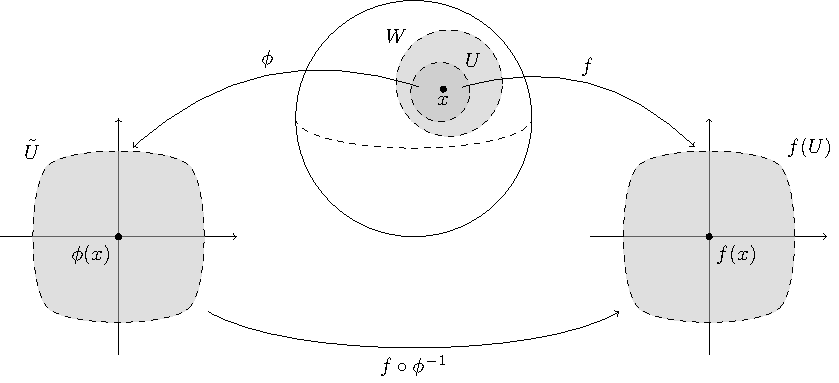
\includegraphics{holomorphic-fct/figure}
	\caption{The function $ f $ is holomorphic (at/on) in line with the function $ f
			\circ \phi ^{-1} $.}
\end{figure*}

\begin{example}
	For a Riemann surface $ X $, with atlas $ \left\{ U _{\alpha}, \phi _{\alpha}
		\right\} $, the charts $ \phi _{\alpha}: U _{\alpha} \to \tilde{U} _{\alpha} $
	are holomorphic on $ U _{\alpha} $.
\end{example}

\begin{example}\label{ex:holo-C-algebra-1}
	Let $ f:X \to \mathbb{C}:x \to z_0 $ for $ z_0 \in \mathbb{C} $ constant. Since
	translative functions are holomorphic in the complex plane, the function $ f $
	is holomorphic at each point $ x \in X $, and hence holomorphic.
\end{example}

\begin{notation}
	It is common to denote the set of holomorphic functions on an open subset $ W
		\subseteq X $ of a Riemann surface $ X $ by $ \mathcal{O}(W) $.
\end{notation}

\begin{proposition}
	$ \mathcal{O}(W) $ is a $ \mathbb{C} $--algebra.
	\begin{proof}
		We recall that for this to be the case, we need that constant functions on $ W $
		are holomorphic, and that sums of holomorphic functions are holomorphic. Since
		the former was shown in Example~\ref{ex:holo-C-algebra-1} we proceed with the
		latter.

		Let $ f,g:W \to \mathbb{C} $ be holomorphic on $ W \subseteq X $, and let $ w
			\in W $. Considering a chart $ (U, \phi) $ at $ w $, and calling on the
		right-distributivity of function composition,
		\begin{align*}
			(f+g)\circ \phi ^{-1}(w) = (f \circ \phi ^{-1})(w) + (g \circ \phi ^{-1})(w)
		\end{align*}
		is a sum of functions which are holomorphic at $ \phi(w) $. The arbitrary
		choice of $ w $ ensures that $ f+g $ is indeed holomorphic on $ W $.
	\end{proof}
\end{proposition}

It is not at all surprising that with the basic definitions supplied, we can
find natural extensions of many results from complex
analysis\sidenote{\footnotesize\cite[p. 29]{miranda}}.

\begin{theorem}[Maximum modulus principle]\label{thm:max-mod}
	Let the function $ f:X \to \mathbb{C} $ be holomorphic on Riemann surface $ X $.
	If there exists a point $ x_0 \in X $ such that, $ |f(x)|\leq|f(x_0)| $ for all
	points $ x \in X $ then $ f $ is constant.
	\begin{proof}
		Suppose that the point $ x_0 $ exists, and consider the set $ \mathcal{X} =
			\left\{ x \in X: f(x)=f(x_0) \right\} $. We can alternatively formulate this set
		as the pre-image of the point $ f(x_0) $, i.e., $ \mathcal{X} = f ^{-1}(f(x_0))
		$, which is closed by the continuity of the function $ f $. Further to this, $
			\mathcal{X} $ is non-empty since $ x_0 \in \mathcal{X} $.

		Let $ \xi \in \mathcal{X} $, and let a chart about the point $ \xi $ be given by
		$ \phi:U \to \tilde{U} $. From the holomorphicity of $ f $ we know that the
		function $ f \circ \phi ^{-1} $ is holomorphic between open subsets of the
		complex plane. Additionally, we have that
		\begin{align*}
			|f(u)|\leq |f(\xi)| \quad \forall u \in U,
		\end{align*}
		which implies,
		\begin{align*}
			|(f \circ \phi ^{-1})(\phi(u))|\leq |(f \circ \phi ^{-1})(\phi(\xi))| \quad
			\forall u \in U.
		\end{align*}
		Then, by the maximum modulus principle (Theorem~\ref{thm:pre-max-mod}) the
		function $ f \circ \phi ^{-1} $ is constant on the connected open subset $
			\tilde{U} $. Consequently,
		\begin{align*}
			f(u) = (f \circ \phi ^{-1})(\phi(u)) = (f \circ \phi ^{-1})(\phi(\xi)) =
			f(\xi) = f(x_0)
		\end{align*}
		for all $ u \in U $, which determines that $ u \in \mathcal{X} $ for all $ u
			\in U $. This is equivalent to $ U \subseteq \mathcal{X} $, and the
		arbitrary choice of $ u $ gives the openness of $ \mathcal{X} $. Since $ X $ is
		connected $ \mathcal{X}=X $, and the statement is proved.
	\end{proof}
\end{theorem}

\begin{corollary}[Liouville]\label{cor:liouville}
	A holomorphic function $ f:X \to \mathbb{C} $ on a compact Riemann surface is
	constant.
	\begin{proof}
		We know that $ |f| $ is a continuous function since $ f $ is holomorphic, and
		the compactness of $ X $ assures that $ |f| $ attains its maximum at some point
		in $ X $. Theorem~\ref{thm:max-mod} determines that the function is constant,
		since $ X $ is connected.
	\end{proof}
\end{corollary}

\begin{example}
	Consider the torus examined in Section~\ref{sec:complex-tori}, $
		\mathbb{C}/\Lambda $, and the related projection map $ \pi:\mathbb{C} \to
		\mathbb{C}/\Lambda $. A function $ f:W \subseteq \mathbb{C}/\Lambda \to
		\mathbb{C} $ is holomorphic at a point $ w \in W $ if and only there exists a
	point $ z \in \pi ^{-1}(w) $ such that $ f \circ \pi $ is holomorphic at $ z $,
	a fact fairly easily observed by considering how we defined the complex charts
	on this space. Furthermore, $ f $ is holomorphic on $ W $ if and only if $ f
		\circ \pi $ is holomorphic on the pre-image of this subset, $ \pi ^{-1}(W) $.

	We now consider the case where $ W = \mathbb{C}/\Lambda $ referring to
	Varolin\sidenotemark. Considering an entire function $ f ^{*} $ we aim to
	determine the necessary criteria such that there exists a function $ f $, as
	above, with $ f ^{*} = f \circ \pi $. In order for this to be the case,
	we need $ f ^{*} $ to be invariant under the action of the lattice $ \Lambda
	$. In other words, we need $ f ^{*}(z) = f ^{*}(z + \lambda) $ for all $
		\lambda \in \Lambda $. Functions with this property are referred to as doubly
	periodic, and by the constancy of $ f $ as a holomorphic function on a compact
	Riemann surface, these functions are constant also.
\end{example}
\sidenotetext[][-9\baselineskip]{\footnotesize\cite{varolin}}

Corollary~\ref{cor:liouville} is perhaps indicative that there is less to
explore in the realm of holomorphic functions on Riemann surfaces, than there
was in the complex plane. Generalisation of another class of functions from
complex analysis proves more fruitful.

\section{Meromorphic functions}\label{sec:mero-fcts}
\begin{definition}[Meromorphicity]
	The complex-valued function $ f:X \to \mathbb{C} $ is said to be
	\defined{meromorphic at} $ x \in X $ if $ f \circ \phi ^{-1} $ is meromorphic
	at $ \phi(x) $, for every chart $ \phi:U \to \tilde{U} $ with $ x \in U $.

	$ f $ is \defined{meromorphic on} $ W \subseteq X $ if it is meromorphic at
	every point $ w \in W $.

	$ f $ is \defined{meromorphic} if it is meromorphic on $ X $.
\end{definition}

\begin{notation}
	It is common to denote the set of meromorphic functions on an open subset $ W
		\subseteq X $ of a Riemann surface $ X $ by $ \mathcal{M}(W) $.
\end{notation}

\begin{example}
	From our definition it is clear that every holomorphic function is meromorphic,
	and hence, for an open subset $ W \subseteq X $, $ \mathcal{O}(W) \subseteq
		\mathcal{M}(W) $.
\end{example}

\begin{example}
	Rational functions on $ \hat{\mathbb{C}} $ are meromorphic.

	We recall that rational functions are those which can be expressed as the
	quotient of polynomials, with denominator not identically $ 0 $. Denoting the
	ring of polynomials functions over $ \mathbb{C} $ by $ \mathbb{C}[z] $, any
	rational function $ f: \hat{\mathbb{C}} \to \mathbb{C} $ can be expressed as
	\begin{align*}
		f(z) = \frac{p(z)}{q(z)},
	\end{align*}
	where $ p \in \mathbb{C}[z] $ and $ q \in \mathbb{C}[z]\setminus \left\{ 0
		\right\} $. The algebraic closedness of $ \mathbb{C} $ determines that both $ p
	$ and $ q $ are entirely factorable;
	\begin{align*}
		\frac{p(z)}{q(z)} = \frac{(z-z _{p_1})\cdots(z-z _{p_m})}{(z-z
		_{q_1})\cdots(z-z _{q_n})},
	\end{align*}
	and hence the function has poles at the points $ z _{q_i} $, while being
	holomorphic away from these points, with some nuance related to cancellation
	of factors.
\end{example}

We can again generalise some well-known results from complex analysis.

\begin{theorem}[Principle of Isolation]
	The zeroes and poles of a meromorphic function $ f:X \to \mathbb{C} $ which is
	not identically zero form a discrete subset of $ X $.
	\begin{proof}
		Suppose that this wasn't the case, and let $ \left\{ x_i \right\} $ be a
		sequence of roots of $ f $ in $ X $ with a limit point $ x \in X $. Then $
			f(x)=0 $ and this is a limit point of the sequence $ \left\{ f(x_i) \right\}
		$ in $ \mathbb{C} $. By the Identity theorem, the function $ f $ must be
		identically $ 0 $. A similar argument for the function $ 1/f $ gives proof
		for the case of the poles.
	\end{proof}
\end{theorem}

\begin{corollary}\label{cor:finite-poles}
	A meromorphic function $ f:X \to \mathbb{C} $ on a compact Riemann surface $ X $
	which is not identically zero has a finite number of zeros and poles.
\end{corollary}

\begin{example}\label{ex:mero-rational-Ch}
	Meromorphic functions on $ \hat{\mathbb{C}} $ are rational.

	Let $ f:\hat{\mathbb{C}} \to \mathbb{C} $ be a meromorphic function.
	Corollary~\ref{cor:finite-poles} allows us to enumerate the zeroes and poles of
	this function. Let there be $ n $ zeroes, with orders $ e_{i} $, and $ m $
	poles with orders $ f_{j} $. If $ m=0 $, $ f $ is holomorphic and hence
	constant by the compactness of $ \hat{\mathbb{C}} $.

	We assume that $ n\geq 1 $ and construct the function
	\begin{align*}
		g(z) = f(z)\cdot \frac{\prod_{i=1}^{n}{(z-z_i)
		^{e_i}}}{\prod_{j=1}^{m}{(z-z_j)^{f_j}}},
	\end{align*}
	which is a meromorphic function of the Riemann sphere without zeroes or poles in
	the complex plane. It must be the case that either $ g $ or $ 1/g $ is
	holomorphic at $ z=\infty $ and hence the $ g(z) = c \in \mathbb{C} $, which
	via algebraic manipulation gives
	\begin{align*}
		f(z) = c\cdot \frac{\prod_{i=1}^{n}{(z-z_i)
		^{e_i}}}{\prod_{j=1}^{m}{(z-z_j)^{f_j}}},
	\end{align*}
	and $ f $ is rational.
\end{example}

The Laurent series of a meromorphic function is an important construction in
complex analysis, and turns out to also be important for meromorphic functions
on Riemann surfaces. If we have a function $ f:X \to \mathbb{C} $ which is
meromorphic at a point $ x \in X $, we can expand the corresponding locally read
meromorphic function $ f \circ \phi ^{-1} $, as a Laurent series. It is
important to note that contrary to the concepts which we have thus far
encountered, the Laurent series of $ f \circ \phi ^{-1} $ \textit{is} dependent
on the choice of chart.

\begin{definition}[Order]
	Let $ f:X \to \mathbb{C} $ be meromorphic at $ x \in X $. The \defined{order}
	of $ f $ at $ x $ is
	\begin{align*}
		\ord(f;x) = \min \left\{ n : c_n \neq 0 \right\},
	\end{align*}
	where $ c_i $ are the coefficients of the local Laurent series of $ f $, i.e.,
	$ f \circ \phi_{x}^{-1} $.
\end{definition}

Initially, the notion of order maybe seems more contrived than it does useful.
It will however have great importance as we reach the latter stages of our
progression, in particular in Chapter~\ref{ch:riemann-roch}. To continue our
exposition of the meromorphic functions on the Riemann sphere, we consider the
following example\sidenote{\footnotesize\cite[p. 27]{miranda}}, which will
undergo generalisation later.

\begin{example}
	A meromorphic function $ f: \hat{\mathbb{C}} \to \mathbb{C} $ is such that
	\begin{align*}
		\sum_{z \in \hat{\mathbb{C}}}^{}{\ord(f;z)}=0.
	\end{align*}

	We know from Example~\ref{ex:mero-rational-Ch} that all meromorphic functions
	can be expressed rationally, and complete factorisation of this rational
	expression gives us that
	\begin{align*}
		f(z) = c \cdot
		\frac{\prod_{i=1}^{n}{(z-z_i)^{e_i}}}{\prod_{j=1}^{m}{(z-z_j)^{f_j}}},
	\end{align*}
	where $ e_i, f_j \in \mathbb{N} $, and $ c \in \mathbb{C}\setminus \left\{ 0
		\right\} $. Alternatively, letting indices range over the integers gives us
	the expression,
	\begin{align*}
		f(z) = c \cdot \prod_{k}^{}{(z-z_k) ^{\alpha_k}.}
	\end{align*}
	We observe that $ \ord(f;z_k) = \alpha_k $, and away from these points the
	only non-zero order is found at $ z= \infty $. In particular, the order at
	this point is given by $ \ord(f; \infty) = \sum_{i}^{}{e_i}- \sum_{j}^{}{f_j}=
		-\sum_{k}^{}{\alpha_k}$. Then,
	\begin{align*}
		\sum_{z \in \hat{\mathbb{C}}}^{}{\ord(f;z)} = \sum_{i}^{}{\alpha_i}-
		\sum_{i}^{}{\alpha_i}=0.
	\end{align*}
\end{example}

\section{Holomorphic maps}
Category theory tells us that a natural next step in our study is the
consideration of maps between our objects of interest. In many ways, the
remaining sections in the chapter provide generalisation of those already seen.
Let $ X $ and $ Y $ be Riemann surfaces with atlases $ \left\{ U, \phi \right\}
$ and $ \left\{ V, \psi \right\} $ respectively.

\begin{definition}[Holomorphicity]\label{def:holomorphic}
	The map $ F:X \to Y $ is said to be \defined{holomorphic at} $ x \in X $ if, for
	all charts $ \phi:U \to \tilde{U} $ with $ x \in U $ and $ \psi: V \to \tilde{V}
	$ with $ F(x) \in V $, the composition
	\begin{align*}
		\psi \circ F \circ \phi ^{-1}: \phi(U \cap V) \to \psi(U \cap V) \\
	\end{align*}
	is holomorphic at $ \phi(x) $.

	$ F $ is \defined{holomorphic on} $ W \subseteq X $ if it is holomorphic at
	every point $ w \in W $.

	$ F $ is \defined{holomorphic} if it is holomorphic on $ X $.
\end{definition}

\begin{figure*}
	\centering
	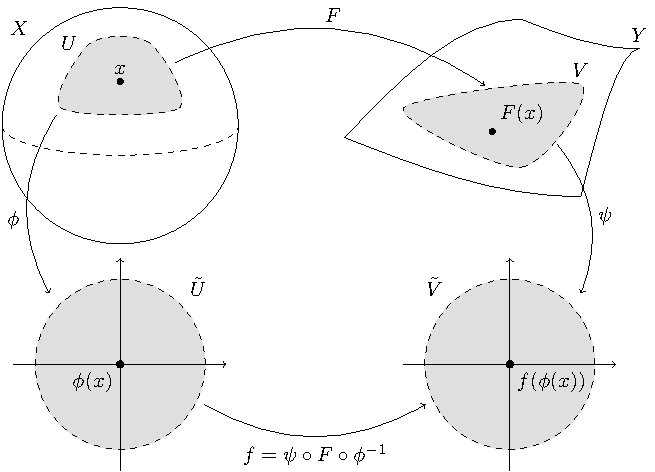
\includegraphics{rs-maps/figure}
	\caption{The map $ F $ is holomorphic if and only if the map $ f $ is
		holomorphic.}
	\label{fig:rs-maps}
\end{figure*}

\begin{remark}
	We have seen that $ \mathbb{C} $ is a non-compact Riemann surface, and hence a
	holomorphic function is simply a holomorphic map to the complex plane.

	It is also worth noting the convention seen in Figure~\ref{fig:rs-maps}. We
	tend to refer to maps specifically between Riemann surfaces by capital
	letters, e.g., $ F $, and the corresponding local representation of the map by
	the corresponding lower case letter, e.g., $ f $.
\end{remark}

\begin{example}\label{ex:holo-id}
	The most basic example is that of the identity map $ \mathrm{id}:X \to X:x
		\mapsto x $. This map is easily seen to be holomorphic since, for any charts $
		\phi_i $ and $ \phi_j $ defined on a neighbourhood of the point $ x $ we have
	that
	\begin{align*}
		\phi_i \circ \mathrm{id} \circ \phi_j ^{-1} & = \phi_i \circ \phi_j ^{-1} \\
		                                            & = \phi _{i,j}
	\end{align*}
	is a transition function, and hence definitively holomorphic.
\end{example}

The fact that identity functions are holomorphic in this
framework allows us to make a further statement, of category theoretic
flavour\sidenote{\footnotesize\cite[p. 39]{miranda}}.

\begin{proposition}
	Riemann surfaces, and the holomorphic maps between them, form a category.
	\begin{proof}
		Example~\ref{ex:holo-id} showed the identity map to be holomorphic, and hence it
		remains to show that the composition of holomorphic maps is holomorphic. Let $
			F:X \to Y $ and $ G:Y \to Z $ be holomorphic maps between Riemann surfaces, $
			X,Y,Z $ with atlases $ \left\{ U, \phi \right\}, \left\{ V, \psi \right\},
			\left\{ W, \sigma \right\} $ respectively.

		Consider a point $ x \in X $, and let $ f = \psi \circ F \circ \phi ^{-1} $
		which is holomorphic at $ \phi(x) $. Let $ y = F(x) $, and let $ g = \sigma
			\circ G \circ \psi ^{-1} $ which is holomorphic at $ \psi(y) $. The composition
		\begin{align*}
			g \circ f & = \left(\sigma \circ G \circ \psi ^{-1}\right)\circ \left( \psi
			\circ F \circ \phi ^{-1} \right)                                            \\
			          & = \sigma \circ G \circ F \circ \phi ^{-1}
		\end{align*}
		is holomorphic at $ \phi(x) $, and the arbitrary choice of $ x $ means that $ G
			\circ F$ is holomorphic.
	\end{proof}
\end{proposition}

Tying the loose ends which we left at the end of
Chapter~\ref{ch:manifold-theory}, we can consider Riemann surfaces to be
equivalent if there exists a bijective holomorphic map with holomorphic inverse
between them\sidenote{\footnotesize\cite[p. 10]{donaldson}}. In this case, we
say that the Riemann surfaces are \defined{biholomorphic}.

\begin{remark}
	An earlier remark made mention of the fact that holomorphic functions are
	nothing more than a specification of holomorphic maps, made by choosing the
	codomain to be $ \mathbb{C} $. A very similar remark can be made for
	meromorphic functions and the Riemann sphere, $ \hat{\mathbb{C}} $.

	Let $ f:X \to \mathbb{C} $ be a meromorphic function, and define a map $ F:X \to
		\hat{\mathbb{C}} $ such that
	\begin{align*}
		F(x) = \begin{cases}
			       f(x)   & \text{if $ x $ is not a pole of $ f $}, \\
			       \infty & \text{if $ x $ is a pole of $ f $}.
		       \end{cases}
	\end{align*}
	This function is holomorphic away from the poles of $ f $ since $ f $ is
	definitively as such. Furthermore, $ F $ is holomorphic at the poles of $ f $
	and thus holomorphic.
\end{remark}

\section{The local model}
It is interesting to note that in our definition of holomorphicity we required
that the local representation of the map was holomorphic with respect to
\textit{every} pair of charts. There is a natural question which arises from
this: are there charts in which the local form is more `nicely' represented than
others? This is indeed the case, and in fact we can make a guarantee on the form
of these local charts in their `nicest' form. Before stating this, we consider
two lemmas which give a complete local description of holomorphic maps on
Riemann surfaces\sidenote{\footnotesize\cite[p. 43]{donaldson}}. Let $ f:U \to
	\mathbb{C} $ be a holomorphic function defined on an open neighbourhood $ U $ of
$ 0 \in \mathbb{C} $, such that $ f(0)=0 $.

\begin{lemma}\label{lem:local-model-1}
	If $ f'(0) \neq 0 $, there exists a neighbourhood $ U' \subset U $ of $ 0 $
	such that $ U' $ is homeomorphic to its image under $ f $, and $ f $ has
	holomorphic inverse on $ U' $.
\end{lemma}

\begin{lemma}\label{lem:local-model-2}
	If $ f \not \equiv 0 $, there exists a unique integer $ m \geq 1 $ and a
	holomorphic function $ g:U' \to \mathbb{C} $ defined on some neighbourhood $
		U' \subset U $ of $ 0 $ such that $ f(z) = g(z)^{m} $ on $ U' $ and $
		g'(0)\neq0 $.
\end{lemma}

\begin{theorem}[Local Normal Form]\label{thm:local-normal-form}
	Let $ F:X \to Y $ be a non-constant holomorphic map between Riemann
	surfaces $ X $ and $ Y $. For any $ x \in X $ there are charts around $ x $,
	and $ F(x)\in Y$ such that the local expression of $ F $ under these charts is
	given by $ z \mapsto z^m $ for some unique integer $ m\geq 1 $.
	\begin{proof}
		Suppose we have a holomorphic map $ F $ as described, and consider the local
		representation of this map in arbitrary charts about a point $ x \in X $ and
		the point $ F(x) \in Y $. We denote this local representation by $ f = \psi
			\circ F \circ \phi ^{-1} $, and apply Lemma~\ref{lem:local-model-2} to find
		a function $ g $ defined on a smaller domain such that $ f = g^m $. We know
		that ther derivative of $ g $ is non-vanishing at $ 0 $, and we can hence
		state, with reference to Lemma~\ref{lem:local-model-1}, that $ g $ is a
		biholomorphism. We can therefore compose $ g $ with the arbitrary charts we
		started with to find charts which have the desired property.
	\end{proof}
\end{theorem}

\begin{marginfigure}[-15\baselineskip]
	\centering
	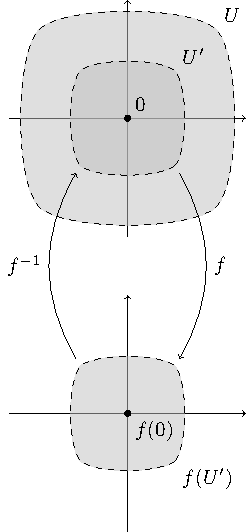
\includegraphics{inverse-fct-thm/figure}
	\caption{Lemma~\ref{lem:local-model-1} is an inverse function theorem type
		statement.}
\end{marginfigure}

We now have a full understanding of the possible holomorphic maps between
Riemann surfaces locally, and the aim of globalising this idea is a natural next
step. Before completing this process, we state yet another generalisation from
complex analysis.

\begin{corollary}[Open Mapping Theorem]
	A non-constant holomorphic map $ F:X \to Y $ is open.
\end{corollary}

\section{Multiplicity and Degree}
In order to globalise this local model of holomorphic maps, we must restrict our
consideration to compact Riemann surfaces.

\begin{definition}[Multiplicity]
	The \defined{multiplicity} of a point $ x \in X $ under a map $ F:X \to Y $ is
	the unique integer $ m $ such that there is a local representation of the map
	as $ z \mapsto z^m $. We denote this by $ \mult(F;x) $.
\end{definition}

\begin{figure*}
	\centering
	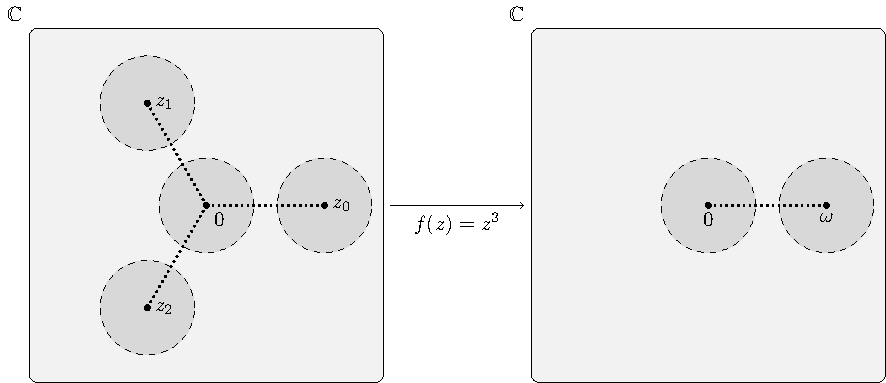
\includegraphics{z^n-degree/figure}
	\caption{The only ramification point is at $ z=0 $.}
	\label{fig:z^n-degree}
\end{figure*}

If $ \mult(F;x) > 1 $, we call $ x $ a \defined{ramification point}, and the
image of a ramification point, is called a \defined{branch point}. Intuition for
these concepts is not hard to come by; consider the entire map $ f:z \mapsto z^3
$, for example. The following explanation will be best understood with relation
to Figure~\ref{fig:z^n-degree}.

In neighbourhoods of each of the points $ z_i \in \mathbb{C}^{*} $, $ z_i $ is
the only point such that $ f(z_i) = \omega $, and so locally, we can represent
this map as constant, and in particular we have that $ \mult(f;z_{i}) = 1 $. Now
consider the point $ 0 \in \mathbb{C} $, and furthermore a neighbourhood $ U $
of $ 0 $. For every point $ u \in U \setminus \left\{ 0 \right\}$ there are two
other points which all, under $ f $, map to the same point. Hence the local
normal form at $ 0 $ is exactly $ z \mapsto z^3 $, and $ \mult(f;0)=3 $. From
this we can see that $ 0 $ is the only ramification point of the map $ f $.

\begin{remark}
	This is a basic, but important example, especially since
	Theorem~\ref{thm:local-normal-form} told us that any map $ F:X \to Y $ can be
	read locally in this way.
\end{remark}

\begin{definition}[Degree]
	The \defined{degree} of a point $ y \in Y $ under a map $ F:X \to Y $ is the
	sum of the multiplicities of points in the pre-image of $ y $. Notatively,
	\begin{align*}
		\deg(F;y) = \sum_{x \in F ^{-1}(y)}^{}{\mult(F;x)}.
	\end{align*}
\end{definition}

\begin{figure*}
	\centering
	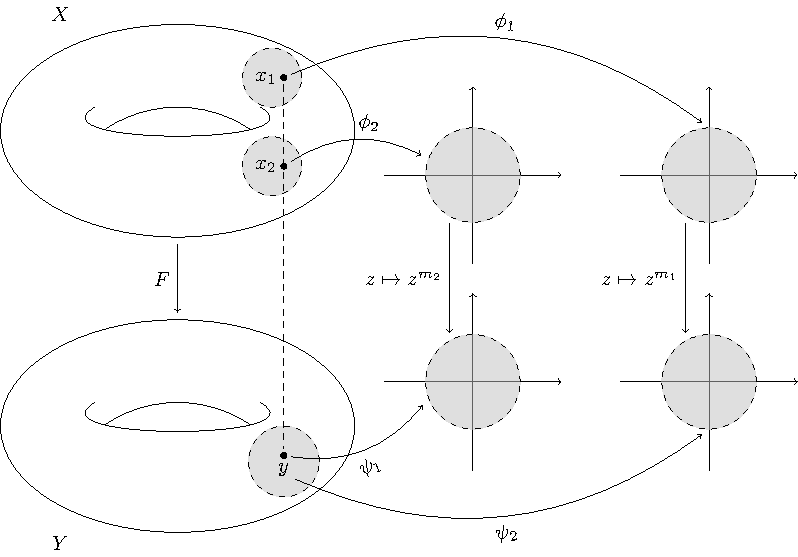
\includegraphics{local-normal-deg-mult/figure}
	\caption{We have that $ \mult(F;x_i)=m_i $ and that $ \deg(F;y)=m_1+m_2 $.}
\end{figure*}

Referring back to the example of $ f:z \mapsto z^3 $, we note that the degree of
the map is constant, since $ \deg(F;\omega)=3 $ for all $ \omega \in \mathbb{C}
$. We can follow a similar line of argument to show the constancy of the degree
under a map $ g:z \mapsto z^n $ for $ n \geq 1 $, and it is natural to question
whether this is a general phenomenon, for all holomorphic maps. This is indeed
the case, as summarised in the following proposition.

\begin{proposition}\label{prop:constant-degree}
	For a non-constant holomorphic map $ F:X \to Y $ between compact Riemann
	surfaces $ X $ and $ Y $, the degree $ \deg(F;y) $ is constant over all $ y \in
		Y$.
\end{proposition}

\begin{notation}
	Motivated by this result, we alter our notation, and refer to the degree of a
	map $ F:X \to Y $ by $ \deg(F) $, removing the dependence on the point in the
	codomain.
\end{notation}

To finish the chapter, we find a relation between the degree of a holomorphic
map between compact Riemann surfaces, and their respective genera. The result is
the Riemann--Hurwitz formula, stated by Riemann, and later proved by Adolf
Hurwitz\sidenote{\footnotesize\cite{hurwitz}}. There are a number of different
proofs of this result, in flavours topological\sidenote{\footnotesize\cite[p.
		100]{donaldson}}, algebraic\sidenote{\footnotesize\cite[p. 90]{griffiths}}, and
analytic\sidenote{\footnotesize\cite[p. 140]{forster}}.

\begin{theorem}[Riemann--Hurwitz Formula]
	Let $ F:X \to Y $ be a non-constant holomorphic map between compact Riemann
	surfaces. Then,
	\begin{align*}
		2 g(X) - 2 = \deg(F) (2 g(Y) - 2) + \sum_{x \in X}^{}{[\mult(F;x)-1]}.
	\end{align*}
\end{theorem}

\begin{example}
	Let $ F(x,y,z)=x^d+y^d+z^d $ and let $ X $ be the associated zero locus in
	projective space. Explicitly,
	\begin{align*}
		X = \left\{ [x:y:z]\in \mathbb{C}\mathbb{P}^{2}: F(x,y,z)=0 \right\}.
	\end{align*}
	We know from Section~\ref{sec:projective-curves}, the homogeneity and
	non-singularity of $ F $ determine that $ X $ is a compact Riemann surface,
	and we aim to compute the genus of this Riemann surface. With $ \pi $ as a
	projection map defined by
	\begin{align*}
		\pi:X \to \mathbb{C}\mathbb{P}^{1}:[x:y:z] \mapsto [x:y],
	\end{align*}
	we call on the fact\sidenotemark\ that a point $ p \in X $ is a ramification
	point under $ \pi $ if and only if $ \partial F/\partial z=0 $. If we
	take $ \alpha = [1:0] \in \mathbb{C}\mathbb{P}^{1} $ it cannot be the case that
	this is a branch point since $ z \neq 0 $ in order that $ \pi ^{-1}( \alpha)
		\subseteq X $. We must have that $ 1+z^d=0 $, and this occurs only at the $ d
	$ roots of unity, all of which are non-zero. Therefore,
	\begin{align*}
		\deg(\pi) = d.
	\end{align*}

	Proposition~\ref{prop:constant-degree} tells us that this is the degree of any
	point in $ \mathbb{C}\mathbb{P}^{1} $. To proceed we consider the point $
		\beta = [1:y] \in \mathbb{C}\mathbb{P}^{1} $ such that $ 1+y^d=0 $. For points
	of this form, it must be the case that pre-images have $ z=0 $, and in
	particular, that $ |\pi ^{-1}(\beta)|=1 $. There are $ d $ solutions to the
	equation $ 1+y^d=0 $, and since every point in $ \mathbb{C}\mathbb{P}^{1} $ can be
	represented in the form $ [1:\gamma] $ for some $ \gamma \in \mathbb{C} $, we
	see that these $ d $ solutions are the only possible branch points in the
	codomain. Applying (and rearranging) the formula, we find that
	\begin{align*}
		g ( X ) = \frac{( d-1 )( d-2 )}{2}.
	\end{align*}
\end{example}

\chapter{Differential forms}\label{ch:differential-forms}
\begin{chout}
	The following chapter gives an exposition of the basics of differential forms
	on manifolds, following Bott--Tu\sidenotemark. In this way, it is written with
	the same motivation as Chapter~\ref{ch:manifold-theory}; we will conclude with
	specification to Riemann surfaces.
\end{chout}
\sidenotetext[][5\baselineskip]{\footnotesize\cite{bott}}

\section{Differential forms on $ \mathbb{R}^{2} $}
Before considering what it means to integrate a function on a Riemann surface,
or even a smooth manifold, we develop the theory of differential forms in the
real plane. Differential forms provide an alternative framework to that of
vector calculus; one which is often considered to be more simple and
flexible\sidenote{\footnotesize\cite{tu}}. Let $ x_1, x_2 $ be the standard
coordinates on $ \mathbb{R}^{2} $ and denote by $ \Omega ^{*} $ the space
generated by $ \d{x_1}, \d{x_2} $, governed by the relations,
\begin{gather*}
	\d{x_i}\d{x_i} = 0,\\
	\d{x_1}\d{x_2} = - \d{x_2}\d{x_1}.
\end{gather*}

\begin{remark}
	The space $ \Omega ^{*} $ can be regarded as a vector space over $ \mathbb{R}
	$, and has the basis,
	\begin{align*}
		1, \d{x_1}, \d{x_2}, \d{x_1}\d{x_2}.
	\end{align*}
\end{remark}

\begin{definition}[Differential forms\sidenotemark]
	With $ \Omega ^{*} $ as above, the \defined{$ C ^{\infty} $ differential forms}
	are elements of,
	\begin{align*}
		\Omega ^{*}\left(\mathbb{R}^{2}\right) = \left\{ C ^{\infty} \text{
			functions on } \mathbb{R}^{2} \right\} \otimes _{\mathbb{R}} \Omega ^{*}
	\end{align*}
	where $ \otimes _{\mathbb{R}} $ denotes the tensor product over $ \mathbb{R}
	$.
\end{definition}
\sidenotetext[][-7\baselineskip]{\footnotesize\cite[p.13]{bott}}

\begin{remark}
	A differential form is simply an expression of the form,
	\begin{align*}
		\omega = \sum_{I}^{}{f _{I} \d{x_I}}
	\end{align*}
	where $ I $ denotes a multi-index, and the $ f_I $ are smooth.
\end{remark}

There is also a natural decomposition (or
grading\sidenote{\footnotesize\cite[p. 13]{bott}}) of the space $ \Omega
	^{*}(\mathbb{R}^{2}) $ as,
\begin{align*}
	\Omega ^{*}( \mathbb{R}^{2}) = \bigoplus_{i=0}^{2}{\Omega
	^{i}(\mathbb{R}^{2})}
\end{align*}
where the space $ \Omega^i(\mathbb{R}^{2}) $ contains the $ i $-forms, over $
	\mathbb{R}^{2} $. To dispense with abstraction, the space $
	\Omega^1(\mathbb{R}^{2}) $ can be recognised as,
\begin{align*}
	\Omega^1(\mathbb{R}^{2}) = \left\{ f(x,y)\d{x} + g(x,y)\d{y}:
	f,g \in C ^{\infty}\left( \mathbb{R}^{2} \right) \right\}.
\end{align*}

Furthermore, we can naturally define a differential operator $ \d{} $ which acts
between these subspaces.

\begin{definition}[Exterior derivative]
	We define the \defined{exterior derivative} to be the differential operator,
	\begin{align*}
		\d : \Omega^i(\mathbb{R}^{2}) \to \Omega ^{i+1}(\mathbb{R}^{2})
	\end{align*}
	with the following conditions.
	\begin{enumerate}
		\item If $ f \in \Omega^0(\mathbb{R}^{2}) $, then,
		      \begin{align*}
			      \d{f} = \frac{\partial f}{\partial x}\d{x} + \frac{\partial f}{\partial
				      y}\d{y}.
		      \end{align*}
		\item If $ \omega \in \Omega ^{*}(\mathbb{R}^{2}) $ can be expressed as $
			      \omega = \sum_{}^{}{f _{I} \d{x_I}} $ for multi-index $ I $,
		      \begin{align*}
			      \d{\omega} = \sum_{}^{}{\d{f_I}\d{x_I}}.
		      \end{align*}
	\end{enumerate}
\end{definition}

\begin{proposition}
	$ \d{}^2=0 $.
	\begin{proof}
		Let us first consider concretely the form of the operator $ \d $ in our
		context. We are given the form of the operator $ d: \Omega^0(\mathbb{R}^{2})
			\to \Omega^1(\mathbb{R}^{2}) $ in the definition, so it remains to consider
		the form of the operator as a function between $ \Omega^1(\mathbb{R}^{2}) $
		and $ \Omega^2(\mathbb{R}^{2}) $.

		Suppose that $ \omega \in \Omega^1(\mathbb{R}^{2}) $, expressible as $ f_1
			\d{x_1} + f_2 \d{x_2} $ for smooth $ 0 $-forms $ f_1,f_2 $. Then,
		\begin{align*}
			\d{\omega} & = \d \left( f_1 \d{x_1} + f_2 \d{x_2} \right)              \\
			           & = \left( \frac{\partial f_1}{\partial x_1}\d{x_1} +
			\frac{\partial f_1}{\partial x_2}\d{x_2} \right)\d{x_1} +
			\left( \frac{\partial f_2}{\partial x_1}\d{x_1} +
			\frac{\partial f_2}{\partial x_2}\d{x_2} \right)\d{x_2}                 \\
			           & = \frac{\partial f_1}{\partial x_2}\d{x_2}\d{x_1} +
			\frac{\partial f_2}{\partial x_1}\d{x_1}\d{x_2}                         \\
			           & = \left( \frac{\partial f_2}{\partial x_1}- \frac{\partial
				f_1}{\partial x_2} \right)\d{x_1}\d{x_2}
		\end{align*}
		using the fact that $ \d{x_1}\d{x_2}= -\d{x_2}\d{x_1} $.

		At this point, we also note that for $ \mathbb{R}^{2} $ the operator $
			\d{}^{2} $ can only act between $ \Omega^0 $ and $ \Omega^2 $. Hence, we
		consider a smooth function $ f $,
		\begin{align*}
			\d{} \circ \d{f} & = \d \left( \frac{\partial f}{\partial x_1}\d{x_1} +
			\frac{\partial f}{\partial x_2}\d{x_2} \right)                             \\
			                 & = \left( \frac{\partial f}{\partial x_1 \partial x_2} -
			\frac{\partial f}{\partial x_2 \partial x_1}\right) = 0
		\end{align*}
		with the final equality a consequence of the interchangeabiliy of partial
		derivatives for smooth functions (Clairaut's Theorem).
	\end{proof}
\end{proposition}

There is another important operation on differential forms, called the
wedge/exterior product, which is easily defined in our framework.

\begin{definition}[Exterior product]
	Let $ \sigma, \tau \in \Omega ^{*}(\mathbb{R}^{2}) $, be representable as $
		\sum_{I}^{}{f_I \d{x_I}} $ and $ \sum_{J}^{}{g_J \d{x_J}} $ for
	multi-indices $ I,J $ respectively. Then, we define the \defined{exterior
		product} of $ \sigma $ and $ \tau $, to be the operation,
	\begin{align*}
		\sigma \wedge \tau = \sum_{I}^{}{f_I \d{x_I}}\wedge \sum_{J}^{}{g_J
		\d{x_J}} = \sum_{I,J}^{}{f_I g_J \d{x_I}\d{x_J}}.
	\end{align*}
\end{definition}

\begin{example}
	We consider the case of $ \sigma, \tau \in \Omega^1(\mathbb{R}^{2}) $. Let $
		\sigma = f_1 \d{x_1}+f_2 \d{x_2} $ and $ \tau = g_1 \d{x_1}+g_2 \d{x_2} $.
	Then,
	\begin{align*}
		\sigma \wedge \tau & = \left( f_1 \d{x_1} + f_2 \d{x_2} \right)\wedge \left(
		g_1 \d{x_1}+ g_2 \d{x_2} \right)                                             \\
		                   & = f_1 g_1 \d{x_1}\d{x_1} + f_1 g_2 \d{x_1}\d{x_2} + f_2
		g_1 \d{x_2}\d{x_1} + f_2 g_2 \d{x_2}\d{x_2}                                  \\
		                   & = f_1 g_2 \d{x_1}\d{x_2} + f_2 g_1 \d{x_2}\d{x_1}       \\
		                   & = \left( f_1 g_2 - f_2 g_1 \right)\d{x_1}\d{x_2}
	\end{align*}
	with each simplification justified by the original defining relations of the
	$ \d{x_i} $.
\end{example}

\subsection{The de Rham complex}
In a somewhat implicit manner, we have introduced a cohomological concept, with
further reaching consequences, than the one we initial desired. The differential
operator $ \d{} $ together with $ \Omega ^{*} $, defines the \defined{de Rham
	complex} on $ \mathbb{R}^{2} $ (and by extension $ \mathbb{R}^{n} $). In a more
general treatment, the de Rham complex is an example of a \defined{differential
	complex} since it can be expressed as a direct sum of vector spaces $ \Omega
	^{*} = \bigoplus_{i=0}^{2}{\Omega^i} $ where there are sequential homomorphisms
defined by the operator $ \d{} $ such that $ \d{}^{2}=0 $.

\begin{marginfigure}
	\centering
	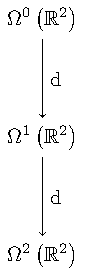
\includegraphics{de-rham/figure}
	\caption{The de Rham complex on $ \mathbb{R}^{2} $.}
\end{marginfigure}

\begin{definition}[de Rham cohomology groups]
	We define the $ i $th \defined{de Rham cohomology group} on $ \mathbb{R}^{n} $
	to be the vector space,
	\begin{align*}
		H^i \left( \mathbb{R}^{n} \right) = \frac{\ker \left( \d{}:
			\Omega^i\left(\mathbb{R}^{2}\right) \to \Omega
			^{i+1}\left(\mathbb{R}^{2}\right) \right)}{\im\left( \d{}: \Omega
			^{i-1}\left(\mathbb{R}^{2}\right) \to
			\Omega^i\left(\mathbb{R}^{2}\right) \right)}.
	\end{align*}
\end{definition}

Of course, we are mostly interested in $ \mathbb{R}^{2} $, and the definition
can be easily specified to this account. We refer to the differential forms
contained in the above kernel as \defined{exact}, and those contained in the
image as \defined{closed}.

\section{Differential forms on smooth manifolds}
Since manifolds are by definition locally Euclidean, we aim to transport our
ideas about differential forms in $ \mathbb{R}^{2} $ into the manifold setting
using the charts and coordinate functions which define the manifold structure.

\begin{definition}[Pullback]
	Let $ u_1, u_2 $ and $ v_1, v_2 $ be standard coordinate systems on two
	subsets $ U, V \subseteq \mathbb{R}^{2} $. For a $ C ^{\infty} $ function $
		f:U \to V $ we define the pullback map $ f ^{*} $ on $ 0 $-forms by,
	\begin{align*}
		f ^{*} & : \Omega^0(V) \to \Omega^0(U) \\
		       & : g \mapsto g \circ f.
	\end{align*}
\end{definition}

So for smooth maps, the pullback is nothing more than pre-composition by a
smooth function. We now aim to extend this idea to forms of higher order, that
is $ 1 $- and $ 2 $-forms. If we impose\sidenote{\footnotesize\cite[p.
		36]{bott}} that the differential operator $ \d{} $ should commute with the
operation of `pulling-back', there is a unique expression of $ f ^{*} $. Letting
$ U, V $ be as in the definition, consider a $ 1 $-form $ \omega \in \Omega^1(V)
$, expressible as $ \omega = \alpha \d{v_1} + \beta \d{v_2}$, for smooth
functions $ \alpha, \beta $. Then the pullback is defined as,
\begin{align*}
	f ^{*} & : \Omega^1(V) \to \Omega^1(U)                                        \\
	       & : \omega \mapsto \left( \alpha \circ f \right) \left( \frac{\partial
		v_1}{\partial u_1}\d{u_1} + \frac{\partial v_1}{\partial u_2}\d{u_2}
	\right)                                                                       \\
	       & \qquad\qquad + \left( \beta \circ f \right) \left( \frac{\partial
		v_2}{\partial u_1}\d{u_1} + \frac{\partial v_2}{\partial u_2}\d{u_2}
	\right).
\end{align*}

\begin{remark}
	Imposing that the operation of pulling-back should commute with the
	differential operator $ \d{} $ is equivalent to the assertion that $ \d{} $ is
	independent of the system of coordinates.
\end{remark}

\begin{definition}[Differential form]
	For a smooth manifold $ M $, defined by an atlas $ \{ U_i, \phi_i \} $, a
	\defined{$ C ^{\infty} $ differential form} is a collection of differential
	forms $ \{ \omega_i \} $, each defined on $ \tilde{U} _{i} $ such that
	\begin{align*}
		U_i \cap U_j \neq \varnothing \implies \phi_i ^{*} \omega_i = \phi_j
		^{*}\omega_j
	\end{align*}
	on the intersection.
\end{definition}

This is an intuitively logical extension of the theory, and while we won't
consider smooth manifolds anymore, $ C ^{\infty} $ forms will remain important,
even in the complex setting.

\section{Differential forms on Riemann surfaces}
Thus far, our development of differential forms has been independent of complex
structure. This complex structure is, however, integral to the definition of
Riemann surfaces and we can use it to further explore differential forms on
manifolds.

To begin with, we change our notation to one more in line with our complex
considerations. Consider a local coordinate $ z = x+iy $, and also the complex
conjugate $ \overline{z} = x - i y $. We can easily invert these relations,
\begin{align*}
	x = \frac{z + \overline{z}}{2},\qquad y = \frac{z - \overline{z}}{2i}
\end{align*}
and can equally well express any $ C ^{\infty} $ $ 1 $-form as,
\begin{align*}
	\omega = f(z, \overline{z}) \d{z} + g(z, \overline{z})\d{\overline{z}}.
\end{align*}

Further to this, we can define the partial differential operators in this
context by,
\begin{align*}
	\frac{\partial }{\partial z} = \frac{1}{2} \left( \frac{\partial }{\partial
		x}-i \frac{\partial }{\partial y} \right), \qquad
	\frac{\partial }{\partial \overline{z}} = \frac{1}{2}\left(
	\frac{\partial }{\partial x}+ i \frac{\partial }{\partial y} \right)
\end{align*}
which have associated differential operators,
\begin{align*}
	\partial = \frac{\partial }{\partial z}\d{z},\qquad
	\overline{\partial} = \frac{\partial }{\partial \overline{z}}\d{\overline{z}}.
\end{align*}

\begin{remark}
	The idea is that the additional complex structure can be summarised as a
	map $ \star: \Omega^1 \to \Omega^1 $ such that
	\begin{align*}
		\star \d{x} = \d{y}, \\
		\star \d{y} = - \d{x}.
	\end{align*}
	From this, we can see that $ \star^2=-1 $, and hence we can decompose the
	space of $ C ^{\infty} $ $ 1 $-forms into the eigenspaces of this operator.
\end{remark}

\begin{lemma}
	For the differential operators $ \d{}, \partial, \overline{\partial} $, we
	have the following identities,
	\begin{gather*}
		\d{} = \partial + \overline{\partial },\\
		\partial ^{2} = \overline{\partial }^{2} = \partial \overline{\partial }+
		\overline{\partial }\partial =0.
	\end{gather*}
\end{lemma}

\begin{notation}
	We denote by $ \Omega ^{1,0}(X) $ the space of differential $ 1 $-forms which
	are locally expressible as $ f(z,\overline{z})\d{z} $, and by $ \Omega
		^{0,1}(X) $ the space of differential forms locally expressible as $ g(z,
		\overline{z})\d{\overline{z}} $.

	This notation is particularly well chosen since it makes clear the fact that
	we are decomposing the space of smooth $ 1 $-forms $ \Omega^1(X) $.
\end{notation}

\begin{marginfigure}
	\centering
	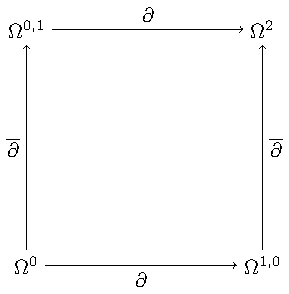
\includegraphics{dolbeault/figure}
	\caption{Visualising the action of $ \partial $ and $ \overline{\partial} $.}
\end{marginfigure}

\begin{definition}[Holomorphic/Meromorphic form]
	A \defined{holomorphic $ 1 $-form} (\defined{meromorphic $ 1 $-form}) on a
	Riemann surface $ X $ is a form which can be locally expressed by,
	\begin{align*}
		\omega = f(z) \d{z}
	\end{align*}
	where $ f $ is holomorphic (meromorphic).
\end{definition}

\begin{definition}[Anti-holomorphic form]
	An \defined{anti-holomorphic $ 1 $-form} on a Riemann surface $ X $ is a form
	which can be locally expressed by,
	\begin{align*}
		\omega = g(z) \d{\overline{z}}
	\end{align*}
	where $ \overline{g(z)} $ is holomorphic.
\end{definition}

\begin{notation}
	It is common to denote the holomorphic $ 1 $-forms on a Riemann surface $ X $
	by $ \mathcal{O}^{1}(X) $, the meromorphic $ 1 $-forms by $
		\mathcal{M}^{1}(X) $, and the anti-holomorphic $ 1 $-forms by $
		\overline{\mathcal{O}^{1}}(X) $.
\end{notation}

There are two results, closely related, which we will need later.

\begin{proposition}\label{prop:hol}
	A smooth function $ f \in \Omega^0(X) $ is holomorphic if and only if $
		\overline{\partial }f=0 $.
	\begin{proof}
		Fixing a local coordinate $ z=x+iy $, we see that
		\begin{align*}
			\overline{\partial }f = 0 \iff
			\frac{\partial f}{\partial \overline{z}} \d{z}=0 \iff
			\frac{\partial f}{\partial x}+i \frac{\partial f}{\partial y}=0,
		\end{align*}
		which are exactly the Cauchy--Riemann equations for $ f $.
	\end{proof}
\end{proposition}

\begin{proposition}\label{prop:anti-hol}
	A smooth function $ g \in \Omega^0(X) $ is anti-holomorphic if and only if $
		\partial g=0 $.
\end{proposition}

These results, can be extended to the holomorphic and anti-holomorphic $ 1
$-forms, and in many cases\sidenote{\footnotesize\cite{forster}} the condition
that $ \overline{\partial }\alpha=0 $ is the defining condition for $ \alpha \in
	\mathcal{O}^{1}(X) $.

Recall that a key integer value associated to a meromorphic map was the order.
We can extend this notion to a meromorphic $ 1 $-forms as follows.

\begin{definition}[Order]
	Let $ p \in X $, $ \omega \in \mathcal{M}^{1}(X) $. Given a local coordinate
	$ z $ centred on $ p $, and a local representation of $ \omega $ as $ f ( z
		)\d{z} $, the \defined{order} of $ \omega $ is defined as,
	\begin{align*}
		\ord ( \omega;p ) = \ord ( f;0 ).
	\end{align*}
\end{definition}

There is a final result\sidenote{\footnotesize\cite[p.132]{miranda}} in the
realm of meromorphic forms and functions which will prove useful.

\begin{lemma}\label{lem:mero-1-forms}
	Let $ \omega_{1}, \omega_{2}\in \mathcal{M}^{1}( X ) $ with $ \omega_{1}
		\not\equiv 0 $. Then, there exists a unique function $ f \in \mathcal{M}( X )
	$ such that
	\begin{align*}
		\omega_{2} = f \omega_{1}.
	\end{align*}
	\begin{proof}
		Suppose that there exists a chart $ \phi:U \to \tilde{U} $ which gives a
		local coordinate $ z $, and suppose also that for $ i=1,2 $, $ \omega_{i} =
			g_{i}(z)\d{z} $, where $ g_{i} $ are meromorphic functions on $ \tilde{U} $.
		If we take $ f = ( g_{2}/g_{1} )\circ \phi $, this is a meromorphic function
		on $ U $, and has the desired property. Showing that this function is
		independent of coordinate chart is straightforward, and this is indeed the
		function we desired.
	\end{proof}
\end{lemma}

\subsection{The Dolbeault complex}
As for the de Rham complex with the differential operator $ \d{} $, we can
define the Dolbeault complex with the operator $ \overline{\partial} $, which
satisfies the conditions for a differential complex since $
	\overline{\partial}\circ\overline{\partial}=0 $. For our consideration, there
will be four particularly important vector spaces.

\begin{gather*}
	H ^{0,0}(X) = \ker \left( \overline{\partial}: \Omega^0 \to \Omega ^{0,1} \right)\\
	H ^{1,0}(X) = \ker \left( \overline{\partial}: \Omega ^{1,0} \to \Omega^2 \right)\\
	H ^{0,1}(X) = \coker \left( \overline{\partial}: \Omega^0 \to \Omega ^{0,1}
	\right) = \left. \Omega^{0}\middle/\im \left( \overline{\partial
	}:\Omega^{0}\to \Omega^{0,1} \right) \right.\\
	H ^{1,1}(X) = \coker \left( \overline{\partial}: \Omega ^{1,0} \to \Omega^2
	\right) = \left. \Omega^{1,0}\middle/\im \left( \overline{\partial }:
	\Omega^{1,0}\to \Omega^{2} \right) \right.
\end{gather*}

The importance of the last two of these spaces is not at all obvious, but the
first two can be easily understood as the spaces of holomorphic functions and
holomorphic $ 1 $-forms.

\section{Integration on Riemann surfaces}
The work of this chapter has all been motivated by the prospect of defining
integration on a Riemann surface, which is what we do now. As in complex
analysis, there are some fundamental results contained in this area. We have
defined the objects we want to integrate, i.e. $ 1 $- and $ 2 $-forms, so we now
define\sidenote{\footnotesize\cite[p. 118]{miranda}} the sets over which we want
to integrate.

\begin{definition}[Path]
	A \defined{path} on a Riemann surface $ X $ is a continuous, piecewise $ C
			^{\infty} $ function,
	\begin{align*}
		\gamma:[a,b]\subseteq \mathbb{R} \to X
	\end{align*}
	where the interval $ [a,b] $ is closed.
\end{definition}

\begin{remark}
	If $ \gamma(a)=\gamma(b) $, we call the path \defined{closed}. We call a path
	\defined{simple} if it is either closed and injective on $ [ a,b ) $, or
	injective.
\end{remark}

\begin{definition}[$ 1 $-form integration]
	Let $ X $ be a Riemann surface, $ \omega $ a $ C ^{\infty} $ $ 1 $-form on $ X
	$, and $ \gamma $ a path whose image is contained by the domain of a single
	chart in the atlas of $ X $, $ \phi:U \to \tilde{U} $. Suppose that $ \omega $
	can be locally represented by $ f \d{z} + g \d{\overline{z}} $ in $ U $. Then,
	the \defined{integral} of $ \omega $ along $ \gamma $ is,
	\begin{align*}
		\int_{\gamma}^{}{\omega} = \int_{\phi \gamma}^{}{f \d{z} + g
		\d{\overline{z}}}
	\end{align*}
	where the right-hand side integral is the standard contour integral.
\end{definition}

\begin{marginfigure}
	\centering
	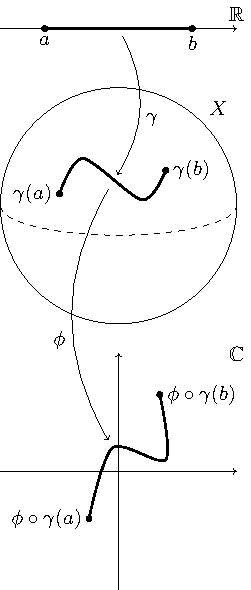
\includegraphics{path/figure}
	\caption{The integral of $ 1 $-form over a path on a Riemann surface.}
\end{marginfigure}

It is fairly clear that any path on a $ X $ may be arbitrarily partitioned, and in
particular, can be partitioned such that each segment of $ \gamma $, is
contained in a single chart of the atlas, i.e., $ \gamma_i \subseteq U_i $. In
this way, we can define the integral of a $ 1 $-form over arbitrary paths on
Riemann surfaces. We also note that the value of this integral is independent of
the choice of partition, since every partition will have some common refinement.

\begin{definition}[Residue]
	Let $ \omega \in \mathcal{M}^{1}(X) $, which has local representation $ f(z)
		\d{z} $ at a point $ p \in X $. Consider a small loop $ \gamma $ in $ X $
	encircling $ p $, then the \defined{residue} of $ \omega $ at $ p $ is,
	\begin{align*}
		\res(\omega;p) = \frac{1}{2 \pi i}\int_{\gamma}^{}{\omega}.
	\end{align*}
\end{definition}

\begin{remark}
	To be exact, by a `small loop' encircling $ p $, we mean a path in $ X $ with
	$ p $ in its interior, containing no other poles of $ \omega $.
\end{remark}

Donaldson\sidenote{\footnotesize\cite[p. 76]{donaldson}} remarks that we may
equally well consider the Laurent series expansion of the local representation
of $ \omega $ as
\begin{align*}
	\omega = f(z) \d{z} = \sum_{j=-k}^{\infty}{a_jz^j} \d{z},
\end{align*}
and take $ \res(\omega;p)=a _{-1} $. This is the route which
Miranda\sidenote{\footnotesize\cite[p. 121]{miranda}} takes. We can of course
show that these two definitions give equivalent formulations. From complex
analysis we know that the residue of a meromorphic function is an important
quantity, and we will soon make a statement of similar intent. First, we
consider what it means to integrate a $ 2 $-form on a Riemann surface.

\begin{definition}[$ 2 $-form integration]
	Let $ X $ be a Riemann surface, $ \rho $ a $ C ^{\infty} $ $ 2 $-form on $ X
	$, and $ T $ a triangular region contained by the domain of a single chart in
	the atlas of $ X $,  $ \phi:U \to \tilde{U} $. Suppose that $ \rho $ has local
	representation $ f(z, \overline{z})\d{z}\d{\overline{z}} $ in $ U $. Then, the
	\defined{integral} of $ \rho $ over $ T $ is,
	\begin{align*}
		\int_{T}^{}{\rho} = \int_{\phi(T)}^{}{f(z,
		\overline{z})\d{z}\d{\overline{z}}}.
	\end{align*}
\end{definition}

\begin{marginfigure}
	\centering
	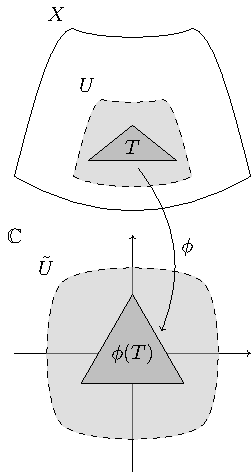
\includegraphics{surface-integral/figure}
	\caption{A integral over the triangular region $ T $ on a Riemann surface.}
\end{marginfigure}

\begin{remark}
	To be pedantic, when we say a triangular region $ T $ on $ X $, we really mean
	the homeomorphic image of some triangular (in the obvious sense) region in the
	complex plane.
\end{remark}

In the multivariate calculus setting there is a relation between the integral
over a region and the integral along the boundary of this region. With the
language of differential forms, we can make analogous statements on Riemann
surfaces. We retain the meaning of $ T $ as a triangular region contained by a
chart domain $ U $ on Riemann surface $ X $ in each of the following results.

\begin{theorem}[Stokes' Theorem]
	Let $ \omega \in \Omega^1(X) $. Then,
	\begin{align*}
		\oint_{\partial T}{\omega} = \int_{T}{\d{\omega}}.
	\end{align*}
	\begin{proof}
		Considering the left-hand side integral as the traversal of the boundary
		counter-clockwise as usual, we can use the definitions of each integral,
		combined with the local representation of the $ 1 $-form $ \omega = f(z,
			\overline{z}) \d{z} + g(z, \overline{z}) \d{\overline{z}} $,
		\begin{align*}
			\oint_{\partial T}{\omega} & = \oint_{\partial \phi(T)}{f(z,
			\overline{z})\d{z} + g(z, \overline{z}) \d{\overline{z}}}           \\
			                           & = \int_{\phi(T)}{\left( \frac{\partial
					g}{\partial z} - \frac{\partial f}{\partial
					\overline{z}} \right)}\d{z}\d{\overline{z}}
			= \int_{T}{\d{\omega}}
		\end{align*}
		where the second equality is justified by Green's theorem in the plane.
	\end{proof}
\end{theorem}

\begin{marginfigure}
	\centering
	\resizebox{\columnwidth}{!}{
		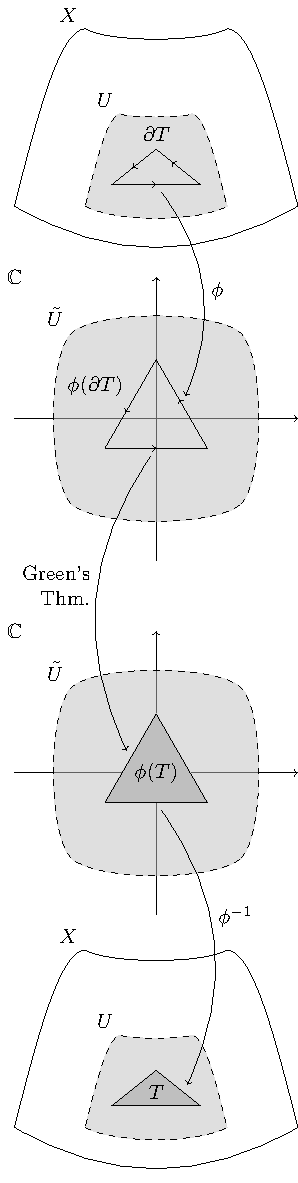
\includegraphics{stokes-theorem/figure}
	}
	\caption{Visualizing the proof of Stokes' theorem.}
\end{marginfigure}

\begin{theorem}[Residue Theorem]
	Let $ \omega \in \Omega^1(X) $ for a compact Riemann surface $ X $. Then,
	\begin{align*}
		\sum_{x \in X}{\res(\omega;x)}=0.
	\end{align*}
	\begin{proof}
		We know that the points at which $ \res(\omega;x) \neq 0 $ are finite, since
		$ X $ is compact, and we hence label these points by $ p_1,...,p_n $. If we
		construct small, simple, closed paths about each of these poles, and denote
		these by $ \gamma_i $, we have by definition that,
		\begin{align*}
			\res(\omega;p_i) = \oint_{\gamma_i}{\omega}.
		\end{align*}
		Furthermore, denote by $ \Gamma_i $ the interior of $ \gamma_i $, and let $
			\Gamma = \bigsqcup_i \Gamma_i$. Then, $ \partial (X \setminus \Gamma) $ is
		the disjoint union of the $ \gamma_i $, and,
		\begin{align*}
			\sum_{i=1}^{n}{\res(\omega;p_i)} & =
			\frac{1}{2 \pi i}\sum_{i=1}^{n}{\int_{\gamma_i}{\omega}}                          \\
			                                 & = \frac{1}{2 \pi i}\int_{\partial (X \setminus
			\Gamma)}{\omega}                                                                  \\
			                                 & = \frac{1}{2 \pi i}\int_{X \setminus
				\Gamma}{\d{\omega}} = 0
		\end{align*}
		with the final equality justified by the fact that $ \d{\omega}=0 $ on $ X
			\setminus \Gamma $, where $ \omega $ is holomorphic, i.e., away from its
		poles.
	\end{proof}
\end{theorem}

\begin{corollary}
	Let $ f $ be a non-constant meromorphic function on compact Riemann surface $
		X$. Then,
	\begin{align*}
		\sum_{x \in X}{\ord(f;x)}=0.
	\end{align*}
	\begin{proof}
		It can\sidenotemark\ be shown that for a non-constant meromorphic function
		$ f $,
		\begin{align*}
			\ord(f;x) = \res \left( \frac{\d{f}}{f};x \right)
		\end{align*}
		for all $ x \in X $. Application of the Residue theorem to the $ 1 $-form $
			\d{f}/f $ gives the result.
	\end{proof}
\end{corollary}
\sidenotetext[][-8\baselineskip]{\footnotesize\cite[p. 80]{forster}}


\chapter{Poisson's Equation}\label{ch:poisson-eq}
\begin{chout}
	We reach the main chapter of the report, and prove\sidenotemark\ a deep,
	analytic result for the to-be-defined Laplacian operator.
\end{chout}
\sidenotetext[][5\baselineskip]{\footnotesize\cite{donaldson}}

\section{Laplace operator}
To give context to the developments of the chapter, it makes sense to state the
result which we ultimately aim to prove. In order to state this result however,
it is necessary to define the Laplacian operator.

\begin{definition}[Laplacian]
	For a Riemann surface $ X $, we define the \defined{Laplacian} to be the
	differential operator
	\begin{align*}
		\Delta: \Omega^0(X) \to \Omega^2(X):f \mapsto 2i
		\overline{\partial}\partial f,
	\end{align*}
	and say that the function $ f $ is \defined{harmonic} if it satisfies,
	\begin{align*}
		\Delta f = 0.
	\end{align*}
\end{definition}

\begin{remark}
	This definition is chosen specifically such that it agrees, in local
	coordinates, with the familiar representation of the Laplace operator as
	\begin{align*}
		\Delta f & = \frac{2i}{4} \left( \frac{\partial }{\partial x}+ i
		\frac{\partial }{\partial y} \right)\left( \frac{\partial }{\partial x}- i
		\frac{\partial }{\partial y} \right) f \d{z}\d{\overline{z}}            \\
		         & = - \left( \frac{\partial^2 }{\partial x^2}+\frac{\partial^2
		}{\partial y^2} \right)f \d{x}\d{y}.
	\end{align*}
\end{remark}

\begin{theorem}\label{thm:fredholm}
	Let $ X $ be a compact Riemann surface and let $ \rho \in \Omega^2(X) $. There
	exists a function $ f \in \Omega^0(X) $ such that $ \Delta f = \rho $ if and
	only if
	\begin{align*}
		\int_{X}{\rho} = 0
	\end{align*}
	and this solution is unique up to an additive constant.
\end{theorem}

The above theorem is referred to as the `Main Theorem' in
Donaldson\sidenote{\footnotesize\cite[p. 113]{donaldson}}. Intuitively, we can
think of this statement as giving the necessary and sufficient conditions to
invert the Laplacian, i.e., solve Poisson's equation, on a compact Riemann
surface.

Initial progress on the proof of Theorem~\ref{thm:fredholm} is easy to come by,
in particular in the `if' direction.

\begin{lemma}
	If there exists a function $ f $ such that $ \Delta f = \rho $,
	\begin{align*}
		\int_{X}{\rho} = 0.
	\end{align*}
	\begin{proof}
		This is a corollary to Stokes' theorem.
		\begin{align*}
			\int_{X}{\rho}  = \int_{X}{\Delta f}
			= 2i \int_{X}{\overline{\partial}\partial f}
			= 2i \int_{X}{\d{\left( \partial f \right)}}
			= 2i \int_{\varnothing}{\partial f} = 0
		\end{align*}
	\end{proof}
\end{lemma}

\begin{lemma}
	If there exists a function $ f $ such that $ \Delta f = \rho $, this function
	is unique up to addition by a constant.
	\begin{proof}
		A simple argument based on maximum modulus principle.
	\end{proof}
\end{lemma}

So, the interesting content in Theorem~\ref{thm:fredholm} can be summarised as
the following.

\begin{theorem}\label{thm:main-thm}
	If $ \rho \in \Omega^2(X) $ is such that
	\begin{align*}
		\int_{X}{\rho} = 0,
	\end{align*}
	there exists a function $ f $ such that $ \Delta f = \rho $.
\end{theorem}

This is the result we aim to prove in the proceeding sections.

\section{Dirichlet norm}
\begin{definition}[$ L^2 $ inner product]
	Let $ \alpha, \beta \in \Omega ^{1,0}(X) $. Then, we define the \defined{$ L^2
		$ inner product} to be,
	\begin{align*}
		\left\langle \alpha, \beta \right\rangle _{L^2} = \int_{X}{i \alpha \wedge
			\overline{\beta}}.
	\end{align*}
\end{definition}

To show that this is definition is more familiar than is superficially obvious,
let us consider a local coordinate $ z=x+iy $ in which $ \alpha $ and $ \beta $
are expressible as $ f(z) \d{z} $ and $ g(z) \d{z} $ respectively. Then,
\begin{align*}
	\left\langle \alpha, \beta \right\rangle _{L^2} & = \int_{X}{i \alpha\wedge
	\overline{\beta}}                                                           \\
	                                                & = i\int_{X}{\left( f(z)
		\d{z} \right)\wedge
		\overline{\left( g(z)\d{z}
	\right)}}                                                                   \\
	                                                & = i\int_{X}{f(z)
	\overline{g(z)}\d{z}\d{\overline{z}}}                                       \\
	                                                & = 2\int_{X}{f
		\overline{g}\d{x}\d{y}},
\end{align*}

and we can define the associated norm,
\begin{align*}
	\|\alpha\|_{L^2}^{2} = \left\langle \alpha,\alpha \right\rangle _{L^2} =
	\int_{X}{i \alpha \wedge \overline{\alpha}} = 2\int_{X}{|f|^{2}\d{x}\d{y}},
\end{align*}
which we refer to as the \defined{$ L^2 $ norm}.

\begin{lemma}
	$ \|\cdot \|_{L^2} $ defines a norm on the compactly supported $ (1,0)
	$-forms.
	\begin{proof}
		There is little to note apart from the fact that compactness ensures the
		finiteness of the defining integral.
	\end{proof}
\end{lemma}

\begin{remark}
	The main observation here is that the $ L^2 $ inner product (and also $ L^{2}
	$ norm) is coordinate independent.
\end{remark}

We can easily extend our definition for the $ L^2 $ inner product (and
consequently norm) to the $ C ^{\infty} $ $ 1 $-forms, by associating these with
their $ (1,0) $ component. In particular, let $ A,B \in \Omega^1(X) $, then,
\begin{gather*}
	\left\langle A,B \right\rangle _{L^2} = 2 \left\langle A ^{1,0}, B ^{1,0}
	\right\rangle _{L^2} = 2i \int_{X}{A ^{1,0}\wedge B ^{0,1}},\\
	\left\|A\right\|_{L^2}^{2} = 2\left\|A^{1,0}\right\|_{L^2}^{2}.
\end{gather*}

\begin{definition}[Dirichlet inner product]
	Let $ f,g:X \to \mathbb{R} $ be $ C ^{\infty} $, at least one compactly
	supported. The \defined{Dirichlet inner product} is defined as
	\begin{align*}
		\left\langle f,g \right\rangle _{\mathcal{D}} = \left\langle \d{f}, \d{g}
		\right\rangle _{L^2},
	\end{align*}
	and similarly, the \defined{Dirichlet norm} is defined as,
	\begin{align*}
		\|f\|_{\mathcal{D}} = \| \d{f}\|_{L^2}.
	\end{align*}
\end{definition}

\begin{remark}
	We note that the Dirichlet `norm' is in fact a `semi-norm', since it is
	positive semi-definite rather than definite. We can see this by noting that
	the constant functions all have zero derivative. As a result of this, it is
	common to consider the space of functions $ C ^{\infty}(X,
		\mathbb{R})/\mathbb{R} $, i.e., the quotient of the space of $ C ^{\infty} $
	functions on $ X $ by the constant functions.
\end{remark}

\begin{lemma}
	If at least one of $ f,g $ have compact support,
	\begin{align*}
		\left\langle f,g \right\rangle _{\mathcal{D}} = \int_{X}{f \Delta g} =
		\int_{X}{g \Delta f}.
	\end{align*}
	\begin{proof}
		Following from the definitions outlined above, and recalling that $ f $ and $
			g$ are real valued gives,
		\begin{align*}
			\left\langle f,g \right\rangle _{\mathcal{D}} & = \left\langle \d{f}, \d{g}
			\right\rangle _{L^2}                                                        \\
			                                              & = 2i \int_{X}{\partial f
				\wedge \overline{\partial
			g}}                                                                         \\
			                                              & = 2i \int_{X}{\partial f
				\wedge \overline{\partial }g}.
		\end{align*}
		Then, integrating by parts gives,
		\begin{align*}
			2i\int_{X}{\partial f \wedge \overline{\partial}g} & = 2i \int_{X}{\partial
				\left( f \overline{\partial}g \right) - f \partial
				\overline{\partial}g}.
		\end{align*}
		Finally, applying Stokes' theorem to the first term in this expression,
		\begin{align*}
			2i \int_{X}{\partial \left( f \overline{\partial}g \right)} - 2i
			\int_{X}{f\partial \overline{\partial}g} & = -2i \int_{X}{f \partial
			\overline{\partial}g}                                                \\
			                                         & = 2i \int_{X}{f
			\overline{\partial}\partial g}                                       \\
			                                         & = \int_{X}{f \Delta g}.
		\end{align*}
	\end{proof}
\end{lemma}

\section{Changing viewpoint}
It is at this point natural to ask how the constructions introduced in the
previous section help us in proving Theorem~\ref{thm:main-thm}. We now dedicate
some time to explore this question in detail, ultimately repackaging the
information contained in Theorem~\ref{thm:main-thm} to something more
appropriate.

To begin, let us denote by $ H $, the space $ C
		^{\infty}(X;\mathbb{R})/\mathbb{R} $, which is an inner product space with
respect to the Dirichlet inner product.

\begin{remark}
	In particular, the inner product $ \left\langle \cdot , \cdot  \right\rangle
		_{\mathcal{D}} $ is positive definite in this case, since the constant functions
	are identified with the class which may be represented by the zero function, $
		\left[ 0 \right] $. Moving forward, we will not make explicit distinction
	between a function $ \psi \in C ^{\infty}(X;\mathbb{R}) $ and the equivalence
	class of functions represented by $ \left[ \psi \right] \in C
			^{\infty}(X;\mathbb{R})/\mathbb{R} $, since this distinction does little
	more than contribute notative complexity to the discussion.
\end{remark}

It is clear that for $ f \in H $, $ \rho \in
	\Omega^2(X) $, the statement $ \Delta f = \rho $ is equivalent to
\begin{align*}
	\int_{X}{g \left( \rho - \Delta f \right)}=0
\end{align*}
for every function $ g \in C ^{\infty}(X ;\mathbb{R}) $. Furthermore,
\begin{align*}
	\int_{X}{g \left( \rho - \Delta f \right)} & = \int_{X}{g \rho} - \int_{X}{g
	\Delta f}                                                                      \\
	                                           & = \int_{X}{g \rho} - \left\langle
	g,f\right\rangle _{\mathcal{D}}.
\end{align*}

Consider now the functional defined by
\begin{align*}
	\tilde{\rho} & : C ^{\infty}(X; \mathbb{R}) \to \mathbb{R} \\
	             & : g \mapsto \int_{X}{\rho g},
\end{align*}
and suppose that $ \int_{X}{\rho} = 0 $ as in the hypothesis of
Theorem~\ref{thm:main-thm}. We claim that this functional descends to a linear
functional on $ H $, which is justifiable by the following. Let $ g \sim g' $ in
$ C ^{\infty}(X;\mathbb{R})/\mathbb{R} $, that is let $ g = g' + c $ for some $
	c \in \mathbb{R}$. Then,
\begin{align*}
	\tilde{\rho}(g) = \int_{X}{\rho g}
	= \int_{X}{\rho \left( g' + c \right)}
	= \int_{X}{\rho g'} + \int_{X}{\rho c}
	= \int_{X}{\rho g'}
	= \tilde{\rho} (g').
\end{align*}

Hence, we define the descended functional,
\begin{align*}
	\hat{\rho} & : H \to \mathbb{R}                          \\
	           & : \left[ g \right] \mapsto \int_{X}{\rho g}
\end{align*}
which allows us to repackage the information contained in
Theorem~\ref{thm:main-thm}.

\addtocounter{definition}{-5}
\begin{theorem}
	If $ \rho \in \Omega^2(X) $ is such that
	\begin{align*}
		\int_{X}{\rho} = 0,
	\end{align*}
	there exists a function $ f $ such that
	\begin{align*}
		\hat{\rho}(g) = \left\langle g,f \right\rangle _{\mathcal{D}}
	\end{align*}
	for all $ g \in H $.
\end{theorem}
\addtocounter{definition}{4}

\section{Riesz representation theorem}\label{sec:riesz}
The previous section seems to have done little for progress aside from change
the framework in which our problem is stated. This is, however, an important
shift, and brings us to a well known result from functional analysis, which will
prove integral.

\begin{theorem}[Riesz representation theorem]\label{thm:riesz}
	Let $ \sigma: \mathcal{H}\to \mathbb{R} $ be a bounded linear function on a
	real Hilbert space $ \mathcal{H} $. Then, there exists an element $ z \in
		\mathcal{H} $, such that
	\begin{align*}
		\sigma(x) = \left\langle z,x \right\rangle
	\end{align*}
	for all $ x \in \mathcal{H} $.
\end{theorem}

Let us now consider the obstacles between our current position and application
of this theorem.
\begin{enumerate}
	\item The functional $ \hat{\rho} $ may not be bounded.
	\item The space $ H $ is not a Hilbert space.
\end{enumerate}

We address these issues in turn.

\subsection{Boundedness of $ \hat{\rho} $}
In order to show the boundedness of $ \hat{\rho} $, we aim to apply a well known
result due to Poincar\'e.

\begin{proposition}[Poincar\'e inequality]\label{prop:poincare-ineq}
	Let $ D \subset \mathbb{R}^{2} $ be a circular disc of area $ A $. Then for $
		\psi $ defined on a superset of $ \overline{D} $, there exists a constant $ C
	$ such that
	\begin{align*}
		\| \psi - \psi_D \|_{L^2 ( D )} \leq C \| \nabla \psi \|_{L^2 ( D )},
	\end{align*}
	where $ \psi_D $ denotes the average of $ \psi $ over $ D $,
	\begin{align*}
		\psi_D = \frac{1}{A}\int_{D}{\psi ( y )}\d{y}.
	\end{align*}
\end{proposition}

\begin{marginfigure}
	\centering
	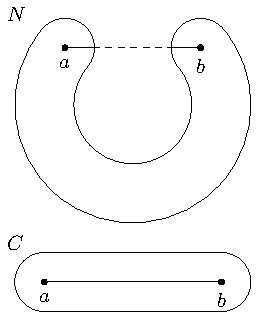
\includegraphics{convex/figure}
	\caption{Proposition~\ref{prop:poincare-ineq} actually holds for any bounded
		convex set $ C $, but we need only consider the case of the disc. Above is a
		convex set $ C $, and a non-convex set $ N $.}
\end{marginfigure}


\begin{remark}
	For reasons related to \defined{partitions of unity} and an isomorphism between
	the second de Rham group and $ \mathbb{R} $, it suffices to show that $
		\hat{\rho} $ is bounded when it is supported in a given chart of the Riemann
	surface\sidenotemark.
\end{remark}
\sidenotetext{\footnotesize\cite[p. 125]{donaldson}}

Let $ (U, \phi) $ be a chart, such that $ \supp \rho \subset U $, and by
homeomorphism identify its image $ \tilde{U} $ with a circular disc $ D $ of
area $ A $. We have a local coordinate system $ ( x,y ) $ on $ D $ afforded to
us by the coordinate map $ \phi $, and in this system, we can consider $ \rho $
as a function of integral $ 0 $, supported on $ D $, and $ \psi $ as a function
(initially on $ X $) defined on some superset of $ \overline{D} $.

These identifications allow us to express the functional in this local
coordinate as
\begin{align*}
	\hat{\rho}( \psi ) = \int_{D}{\rho \psi}\d{x}\d{y},
\end{align*}
which is equivalently expressed as
\begin{align*}
	\hat{\rho}( \psi ) = \int_{D}{\rho ( \psi - \psi_D )}\d{x}\d{y},
\end{align*}
since the integral of $ \rho $ is zero. This is exactly, the form (up to
scaling) of the $ L^2 $ norm introduced earlier, and as such, we can utilise the
Cauchy-Schwarz inequality to state that,
\begin{align*}
	\left| \int_{D}{\rho ( \psi-\psi_D )}\d{x}\d{y} \right| \leq \| \rho
	\|_{L^2(D)}\| \psi-\psi_D \|_{L^2(D)}.
\end{align*}
A final series of relations, the first justified by
Proposition~\ref{prop:poincare-ineq}, and the last by definition,
\begin{align*}
	| \hat{\rho}( \psi ) | \leq C \| \nabla \psi \|_{L^2 ( D )}
	\leq \| \nabla \psi \|_{L^2 ( X )} = C \| \psi \|_{\mathcal{D}}
\end{align*}
proves the boundedness of the functional in $ U $ and, by the above remark, on
$ X $.

\subsection{Completion}
We know that the functional $ \hat{\rho} $ is bounded, and hence it remains to
find a Hilbert space which is related to $ H $. We do this via the abstract
completion.

\begin{definition}[Completion]
	For an inner product space $ H $, with the inner product $ \left\langle \cdot
		,\cdot \right\rangle $ and the associated norm $ \|\cdot \| $, the
	\defined{completion} of $ H $ with respect to $ \| \cdot \| $, is a set of
	equivalence classes of Cauchy sequences $ \left( g_i \right) \in H $ where,
	\begin{align*}
		\left( g_i \right)\sim \left( g_i' \right) \iff \|g_i - g_i'\| \to 0.
	\end{align*}
\end{definition}

We denote by $ \mathcal{H} $ the completion of $ H $ with respect to the
Dirichlet norm $ \|\cdot\|_{\mathcal{D}} $. At this stage, application of the
Riesz representation theorem is obstructed solely by the fact that our
functional $ \hat{\rho} $ is defined on $ H $, rather than $ \mathcal{H} $. The
following result helps us solve this minor issue.

\begin{lemma}
	Let $ U,V $ be two normed spaces with respective norms $ \|\cdot \|_{U} $ and
	$ \|\cdot \|_{V} $, and consider the linear map $ \sigma:U \to V $. If $
		\sigma $ is bounded, then $ \sigma(u_i) $ is a Cauchy sequence in $ V $ for
	any Cauchy sequence $ (u_i) $ in $ U $.
	\begin{proof}
		We recall that the boundedness of the linear map $ \sigma $ is definitively
		equivalent to the existence of a constant $ C $ such that
		\begin{align*}
			\|\sigma(u)\|_{V} \leq C \|u\|_{U}
		\end{align*}
		for all $ u \in U $. Since $ (u_i) $ is Cauchy,
		\begin{align*}
			\|u_n - u_m\|_{U} \to 0
		\end{align*}
		as $ n,m \to \infty $, and hence
		\begin{align*}
			\|\sigma(u_n) - \sigma(u_m)\|_{V} & = \|\sigma(u_n-u_m)\|_{V}    \\
			                                  & \leq C \|u_n-u_m\|_{U} \to 0
		\end{align*}
		as $ n,m \to \infty $.
	\end{proof}
\end{lemma}

In our setting, this result determines that the sequence $ \hat{\rho}(g_i) $ is
Cauchy in $ \mathbb{R} $, and hence convergent. As a result, we can define the
extension of $
	\hat{\rho} $ by,
\begin{align*}
	\hat{\rho} & : \mathcal{H} \to \mathbb{R}                             \\
	           & : [(g_i)] \mapsto \lim _{i \to \infty}{\hat{\rho}(g_i)},
\end{align*}
which is a bounded linear map as needed. We choose to denote the extended
functional in the same way as the original functional, since these are so
closely related. Finally, we are in a position to apply Theorem~\ref{thm:riesz},
and can assert the existence of $ f \in \mathcal{H} $ such that
\begin{align*}
	\hat{\rho}(g) = \left\langle f,g \right\rangle _{\mathcal{D}}
\end{align*}
for all $ g \in \mathcal{H} $. A solution of this type is called a \defined{weak
	solution}, and for the proof of Theorem~\ref{thm:main-thm} we must show that
this weak solution is in fact a valid, smooth solution.

\section{Weyl's Lemma}
The following section concerns itself with the proof of a version of Weyl's
lemma, which will tie up the proof of Theorem~\ref{thm:main-thm}, in that it
will determine that any weak solution is smooth.

\begin{proposition}[Weyl's Lemma]\label{prop:weyl}
	Let $ D \subseteq \mathbb{C} $ be a bounded, open set, and let $ \rho \in
		\Omega^2(D) $. If $ \phi \in L^{2}(D) $, such that
	\begin{align*}
		\int_{D}{\chi \Delta \phi} = \int_{D}{\chi \rho}
	\end{align*}
	for all compactly supported, smooth functions $ \chi $, $ \phi $ is smooth,
	and satisfies $ \Delta \phi = \rho $.
\end{proposition}

\subsection{Relation to an $ L^{2} $ function}
To reiterate our current position, we have found a weak solution to the Posson
equation, $ f \in \mathcal{H} $ which is a Cauchy sequence $ ( f_{i} ) $ with
respect to $ \| \cdot  \|_{\mathcal{D}} $ such that, for any $ g $,
\begin{align*}
	\left\langle f_{i},g \right\rangle \to \hat{\rho}( g )
\end{align*}
as $ i \to \infty $. In order to apply Proposition~\ref{prop:weyl} we aim to
associate the Cauchy sequence with a locally $ L^{2} $ function. We first
consider this association in a single coordinate chart $ ( U, \phi ) $, and
identify $ \phi ( U ) $ with a bounded open set $ D \subseteq \mathbb{C} $.
Since the underlying collection of functions $ H $ of our completion $
	\mathcal{H} $ is $ C^{\infty}( X;\mathbb{R} )/\mathbb{R} $, we may freely add
constants to the functions $ f_{i} $ such that their integral vanishes over the
region $ D $. In particular, we can ensure that the average $ [ f_{i} ]_{D}=0 $.
Then,
\begin{align*}
	\left\| f_{n}-f_{m} \right\|_{L^{2}(D)} & = \left\| f_{n}-f_{m} -
	[ f_{n}-f_{m} ]_{D} \right\|_{L^{2}(D)}                                       \\
	                                        & \leq \left\| \nabla ( f_{n}-f_{m} )
	\right\|_{L^{2}(D)}                                                           \\
	                                        & \leq \left\| f_{n}-f_{m}
	\right\|_{\mathcal{D}} \to 0
\end{align*}
as $ n,m \to \infty $,which is enough to declare $ ( f_{i} ) $ as Cauchy in $
	L^{2} $. Furthermore, since $ L^{2}(D) $ is complete, $ ( f_{i} ) $ converges to
some function $ f \in L^{2}(D) $.

\begin{lemma}
	The sequence of functions $ ( f_{i} ) $ converges locally in $ L^{2} $ on $ X $.
	\begin{proof}
		We now aim to extend our above argument to account for all coordinate
		charts.

		Let $ A $ be the collection of points $ x \in X $ such that there exists a
		coordinate chart $ U_{x} $ in which $ \phi_{i}\to \phi$ with respect to $
			\|\cdot \|_{L^{2}} $. $ A $ is by nature open, and non-empty by the previous
		argument. Furthermore, $ X $ is connected, and hence, we aim to show that $
			A $ is closed, determining that $ A=X $.

		To proceed by contradiction, let us suppose that $ A $ is not closed.
		Taking, $ x \in \overline{A}\setminus A $, and a neighbourhood $ U_{x} $ of
		$ x $, we see that in the same way as above, there exists a sequence of real
		numbers $ ( c_{i} ) $ such that $ ( f_{i}-c_{i} ) $ converges in $ L^{2}(
			U_{x} ) $. For any $ y \in A \cap U_{x} $, both $ ( f_{i}-c_{i} ) $ and $
			( f_{i} )$ converge, and this forces that $ c_{i}\to 0 $, since these
		limits must equate as $ i \to \infty $. This determines that $ x $ is in
		fact in $ A $, which gives the desired contradiction.
	\end{proof}
\end{lemma}

The outcome of the subsection is that we now have a function $ f $ on $ X $
which is locally square-integrable, and a weak solution to $ \Delta f = \rho $.

\subsection{The Newton potential}
To proceed with the proof of Proposition~\ref{prop:weyl}, we consider the case
where $ \rho=0 $, i.e., the case where the $ L^{2} $ function $ f $ is
harmonic. We note also that since smoothness is a local
property\sidenote{\footnotesize\cite[p. 127]{donaldson}}, we can further reduce
our consideration to any interior set $ D' $ such that the $ \epsilon
$-neighbourhood of $ D' $ is contained by $ D $. For this case, a first
necessary introduction is the Newton potential.

\begin{marginfigure}[-2\baselineskip]
	\centering
	\resizebox{\columnwidth}{!}{
		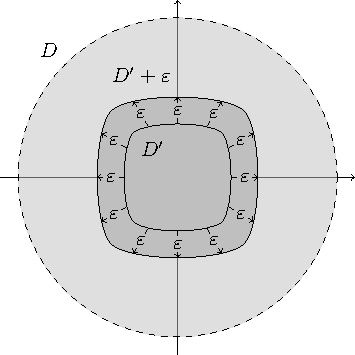
\includegraphics{interior-set/figure}
	}
	\caption{The $ \epsilon $-neighbourhood of $ D' $ is contained by $ D $.}
\end{marginfigure}

\begin{definition}[Newton potential]
	The \defined{Newton potential} is the function
	\begin{align*}
		K(x) = \frac{1}{2 \pi}\log | x |.
	\end{align*}
\end{definition}

\begin{remark}
	We make a brief note of the fact that for any smooth function $ g $ which is
	compactly supported in $ \mathbb{C} $, the convolution $ K*g $ is smooth.
\end{remark}

There is a very close relation between $ K(x) $, and the operator $ \Delta $.
This is well summarised by the following standard result.

\begin{lemma}\label{lem:inverse-laplacian}
	Let $ \sigma $ and $ \tau $ be compactly supported in $ \mathbb{C} $. Then,
	\begin{gather*}
		K* ( \Delta \sigma ) = \sigma,\\
		\Delta ( K*\tau ) = \tau.
	\end{gather*}
\end{lemma}

\begin{remark}
	This result is pertinent since it essentially states that convolution with
	the Newton potential $ K $, is inverse to operation by $ \Delta $.
\end{remark}

We recall the mean value property of harmonic
functions\sidenote{\footnotesize\cite[p. 237]{rudin}}, states that a smooth
harmonic function $ \phi $ defined on the neighbourhood of $ D' $ centered at $
	0 $, is such that,
\begin{align*}
	\phi ( 0 ) = \phi_{\partial D'}.
\end{align*}

Consider a smooth \defined{cutoff} function $ \beta:[0, \infty) \to \mathbb{R} $
defined such that it is constant for small $ r $, and zero for $ r > \epsilon $,
where $ \epsilon>0 $ is fixed. Furthermore, let $ \beta $ be normalized such
that,
\begin{align*}
	2 \pi\int_{0}^{\infty}{r \beta ( r )}\d{r} = 2 \pi\int_{0}^{\epsilon}{r \beta
		( r )}\d{r} = 1.
\end{align*}
We now define a related function $ B:z \mapsto \beta ( | z | ) $. It is clear
that $ B $ is smooth, and we can also show that it has integral $ 1 $ over $
	\mathbb{C} $,
\begin{align*}
	\int_{\mathbb{C}}{B ( z )}\d{z} = \int_{\mathbb{C}}{\beta ( | z | )}\d{z} =
	\int_{0}^{2 \pi}{\int_{0}^{\infty}{r \beta ( r )}\d{r}}\d{\theta} = 1.
\end{align*}

\begin{lemma}
	If $ f $ is a smooth, harmonic function on $ D' $, then $ B * f = f $.
	\begin{proof}
		Translation invariance allows us to treat only the case where $ z=0 $. In
		this scenario,
		\begin{align*}
			B * f ( 0 ) & = \int_{\mathbb{C}}{B ( -z )f ( z )}\d{z}               \\
			            & = \int_{0}^{\infty}{\int_{0}^{2 \pi}{r \beta ( r )f ( r
			e^{i \theta})}\d{\theta}}\d{r}                                        \\
			            & = 2 \pi f ( 0 )\int_{0}^{\infty}{r \beta ( r )}\d{r}    \\
			            & = f ( 0 ).
		\end{align*}
	\end{proof}
\end{lemma}

\begin{corollary}\label{cor:B-convolution}
	Let $ J \subset \mathbb{C} $ be compact, and let $ f $ be a smooth function
	on $ \mathbb{C} $ such that $ \supp \Delta f \subset \mathbb{C} $. Then $
		B*f = f $ outside the $ \epsilon $-neighbourhood of $ J $.
\end{corollary}

At this point, the remainder of the argument is clear. We can combine the
previous lemma, with what we know about the convolution as follows. If the
function $ f $ is smooth on $ D $, we must have that $ B * f = f $ on any smooth
interior domain $ D' $ of $ D $. Furthermore, we know that for any $ L^{2} $
function $ g $, $ B*g $ is smooth. As a result, there is an equivalence between
proving the smoothness of $ f $ in $ D' $ and showing that $ B*f=f $ in this
domain.

Let $ \chi $ be a smooth function such that $ \supp \chi \subset D' $. We aim to
show that given this arbitrary choice of function,
\begin{align*}
	\langle \chi, f - B*f \rangle_{L^{2}( D' )}=0,
\end{align*}
using the fact\sidenote{\footnotesize\cite[p. 129]{donaldson}} that $ \langle a,
	b*c \rangle = \langle b*a, c \rangle $. Then, dropping the subscript for
brevity,
\begin{align*}
	\langle \chi, f-B*f \rangle = \langle \chi,f \rangle - \langle B*\chi, f
	\rangle = \langle \chi-B*\chi,f \rangle.
\end{align*}

We know from Lemma~\ref{lem:inverse-laplacian} that $ \Delta ( K * \chi )=\chi
$, and hence $ \supp \Delta ( K * \chi ) = \supp \chi \subseteq D' $. As a
result, we can apply Corollary~\ref{cor:B-convolution} to state that $ B* ( K*
	\chi ) = K*\chi $ outside $ D' $. Now, let $ h = K* \chi - B*K*\chi = K*( \chi
	- B*\chi) $, which by the previous arguments is compactly supported in $ D $.
Since $ f $ is a weak solution, we have that, $ \langle \Delta h, f \rangle =
	0 $, and rearranging, we have that,
\begin{align*}
	\langle \Delta h,f \rangle=0 \iff \langle \Delta ( K* ( \chi - B*\chi ) ), f \rangle=0
	\iff \langle \chi - B*\chi, f \rangle=0.
\end{align*}

The final piece in the proof of Proposition~\ref{prop:weyl} is to show that
this is sufficient to state that $ f $ is smooth on $ D $ for any $ \rho \in
	\Omega^{2}( D ) $. For any $ \rho $, we can choose some $ \rho' $ which is
equal to $ \rho $ on a neighbourhood of $ D' $ and compactly supported on $ D
$. We can find a weak solution $ f' = K* \rho' $ to $ \Delta f' = \rho' $ on $
	D $, which we know to be smooth. Then, the smoothness of $ f $ is equivalent to
the smoothness of $ f-f' $, and since we know that $ \Delta ( f - f' ) = \rho -
	\rho' = 0 $ on $ D $, this must be the case.

With the proof of Proposition~\ref{prop:weyl} comes also the proof of
Theorem~\ref{thm:main-thm}, and we can move onto the consequences of this
fundamental analytic result.

\chapter{Riemann--Roch Theorem}\label{ch:riemann-roch}
\begin{chout}
	With the conditions for inversion of the Laplacian behind us, we now prove the
	famous Riemann--Roch theorem.
\end{chout}

\section{Divisors}
In order to state the Riemann--Roch theorem, we first introduce the notion of a
divisor\sidenote{\footnotesize\cite[p. 129]{miranda}}. While initially an
abstract construction, divisors will allow us to jointly consider the zeros and
poles of a meromorphic function.

\begin{definition}[Divisor]
	A \defined{divisor} on a Riemann surface $ X $ is a function $ D:X \to
		\mathbb{Z} $ which has discrete support in $ X $.
\end{definition}

With the introduction of a formal summation notation, the idea of a divisor
become clearer. In particular, it is common to denote a divisor $ D $ by
\begin{align*}
	D=\sum_{p \in X}^{}{D(p) \cdot p},
\end{align*}
where $ D(p) \neq 0 $ only on a discrete subset of $ X $.

\begin{remark}
	We make an initial remark that in the same way as the discreteness of zeroes of
	meromorphic functions on all Riemann surfaces determined the finiteness of
	zeroes on \textit{compact} Riemann surfaces, the support of a divisor on a
	compact Riemann surface is necessarily finite.
\end{remark}

This remark is important, since it allows us to remove the formality of the sum
in construction of the following.

\begin{definition}[Degree]
	Let $ D $ be a divisor on a compact Riemann surface. The \defined{degree} of
	$ D $ is the sum of its values,
	\begin{align*}
		\deg(D) = \sum_{p \in X}^{}{D(p)}.
	\end{align*}
\end{definition}

There will be two particularly important examples of divisors for our
progression towards the Riemann--Roch theorem; those related to meromorphic
functions and $ 1 $-forms.

\begin{definition}[Principal divisor]
	A divisor is said to be \defined{principal} if it can be associated to the
	order of a meromorphic function,
	\begin{align*}
		(f) = \sum_{p \in X}^{}{\ord(f;p)\cdot p}.
	\end{align*}
\end{definition}

\begin{example}
	We have completely classified the meromorphic functions on the Riemann sphere
	as the rational functions, and aim to determine a general form for the
	principal divisor associated to these functions. Let
	\begin{align*}
		f(z) = c \cdot
		\frac{\prod_{i=1}^{n}{(z-z_i)^{e_i}}}{\prod_{j=1}^{m}{(z-z_j)^{f_j}}}
	\end{align*}
	be a general rational function on $ \hat{\mathbb{C}} $. Then,
	\begin{align*}
		\left( f \right) = \sum_{i=1}^{n}{e_i \cdot z_i} - \left(
		\sum_{j=1}^{m}{f_j} \right)\cdot \infty,
	\end{align*}
	since the function has zeroes of order $ e_i $ at the points $ \left\{ z_i
		\right\} $ and poles of order $ f_j $ at the points $ \left\{ z_j \right\} $.
\end{example}

\begin{definition}[Canonical divisor]
	A divisor is said to be \defined{canonical} if it can be associated to the
	order of a meromorphic $ 1 $-form,
	\begin{align*}
		(\omega) = \sum_{p \in X}^{}{\ord(\omega;p)\cdot p}.
	\end{align*}
\end{definition}

\begin{remark}
	It is common to denote the set of all divisors on a Riemann surface $ X $ by
	$ \mathrm{Div}(X) $, and this is in fact a group under pointwise addition.
	Furthermore, it follows directly from the definition that for $ f,g \in
		\mathcal{M}(X)\setminus \left\{ 0 \right\} $,
	\begin{gather*}
		(f g) = (f) + (g), \\
		(f/g) = (f) - (g), \\
		(1/f) = -(f),
	\end{gather*}
	and in particular, the principal divisors form a subgroup of $ \mathrm{Div}(X)
	$.
\end{remark}

It is logical now to make an attempt to organise the divisors, and in this vein,
we introduce a partial ordering. In particular, $ D \geq 0 $ if $ D(p) \geq 0
$ for all $ p $, and $ D \geq D' $ if $ D - D' \geq 0 $. From this partial
ordering, we can define\sidenote{\footnotesize\cite[p. 146]{miranda}} some
notable spaces of divisors.

\begin{definition}
	The space of meromorphic functions which have poles bounded by the divisor $ D
	$ is denoted and defined as,
	\begin{align*}
		L(D) = \left\{ f \in \mathcal{M}(X): (f) + D \geq 0 \right\}.
	\end{align*}
\end{definition}

Understanding of this space is most easily obtained by considering a single
point $ x \in X $. Suppose the divisor $ D $ is such that $ D(x) = n > 0 $.
Then, the condition that $ f \in L(D) $, is that $ (f) + D \geq 0 $ at $ x $,
which is in turn that $ \ord(f;x) + n \geq 0 $, i.e., the function $ f $ can
have a pole of at \textit{most} order $ n $ at the point $ x $.

Now consider the alternative, that $ D(x) = -n < 0 $. Then, with the same
logic as previously, $ \ord(f;x) - n \geq 0 $, and in particular, $ f $ must
have a zero of at \textit{least} order $ n $ at the point $ x $.

\begin{remark}
	If we take $ D $ to be the trivial divisor, then the space of meromorphic
	functions bounded by this divisor is exactly the space of holomorphic
	functions. That is,
	\begin{align*}
		L(0) = \mathcal{O}(X)
	\end{align*}
	which is the space of constant functions for any compact $ X $.
\end{remark}

We could choose to define an analogous space for the meromorphic $ 1 $-forms,
although this would be unnecessary. Recall that by Lemma~\ref{lem:mero-1-forms},
two non-zero $ 1 $-forms are multiplicatively related by a unique meromorphic
function. Therefore, for a canonical divisor $ K= (\omega) $, the space
\begin{align*}
	L(K-D) & = \left\{ f \in \mathcal{M}(X): (f) + K - D \geq 0 \right\}        \\
	       & = \left\{ f \in \mathcal{M}(X): (f) + (\omega) - D \geq 0 \right\} \\
	       & = \left\{ f \in \mathcal{M}(X): (f \omega) - D \geq 0 \right\}     \\
	       & = \{ f \omega \in \mathcal{M}^{1}(X): (f \omega) - D \geq 0 \}
\end{align*}
is exactly the analogous construction we wanted.

\section{Cohomological precursors}
Historically, the Riemann--Roch theorem came to fruition in two
parts\sidenote{\footnotesize\cite[p. 192]{miranda}}. Riemann found a lower bound
for the dimension of $ L ( D ) $, and it was Riemann's student, Roch, who
provided the term needed for equality. We will approach our consideration of
this result in the same manner, but it is first necessary to prove some results
related to the cohomological concepts we introduced in
Chapter~\ref{ch:differential-forms}.

\begin{lemma}
	The map
	\begin{align*}
		i:\overline{\mathcal{O}^{1}}(X) \to H ^{0,1}(X):\omega \mapsto [ \omega ]
	\end{align*}
	is an isomorphism.
	\begin{proof}
		Firstly, we show that $ i $ is injective; in particular that $ \ker(i) $
		is trivial. To do this, consider an element $ [ \omega ]\in H ^{0,1}(X) $
		such that $ [ \omega ]=0 $. By the definition of the cokernel, this means
		that there exists some smooth function $ f \in \Omega^0(X) $ such that
		\begin{align*}
			\overline{\partial }f          & = \omega,          \\
			\partial \overline{\partial }f & = \partial \omega.
		\end{align*}
		By Proposition~\ref{prop:anti-hol}, we know that $ \partial \omega=0 $, and
		in particular,
		\begin{align*}
			\Delta f = 0.
		\end{align*}
		By Theorem~\ref{thm:main-thm} this function $ f $ must be unique up to
		additive constant, and since $ \Delta 0 = 0 $, $ f $ must be constant. This
		determines that
		\begin{align*}
			0 = \overline{\partial }f = \omega,
		\end{align*}
		hence $ \ker(i) $ is trivial, and $ i $ is injective.

		Now, to show that $ i $ is surjective, consider an element $ [ \theta ]\in H
				^{0,1}(X) $. We need to find an element $ \omega \in
			\overline{\mathcal{O}^{1}}(X) $ such that $ i ( \omega ) = [ \theta ] $ that
		is, we need to find a smooth function $ \phi $ such that,
		\begin{align*}
			\omega = \theta + \overline{\partial }\phi.
		\end{align*}
		This is equivalent to,
		\begin{align*}
			\partial \omega & = \partial \theta + \partial \overline{\partial }\phi \\
			0               & = \partial \theta + \partial \overline{\partial }\phi \\
			\Delta \phi     & = 2i\partial \theta.
		\end{align*}
		Since
		\begin{align*}
			\int_{X}{\partial \theta} = \int_{X}{\d{\theta}} = \int_{\partial
				X}{\theta}=0,
		\end{align*}
		Theorem~\ref{thm:main-thm} determines the existence of $ \phi $.
	\end{proof}
\end{lemma}

\begin{remark}
	This provides some unification of our understanding. It was clear that $
		\mathcal{O}^{1}(X) \cong H ^{1,0}(X) $, and we know have that $
		\overline{\mathcal{O}^{1}}(X) \cong H ^{0,1}(X) $.
\end{remark}

\begin{lemma}
	The map
	\begin{align*}
		v: \mathcal{O}^{1}(X) \oplus \overline{\mathcal{O}^{1}}(X) \to H^1(X): (
		\omega_1, \omega_2 ) \mapsto [ \omega_1+\omega_2 ]
	\end{align*}
	is an isomorphism.
	\begin{proof}
		The proof uses a similar strategy to that employed for the previous lemma,
		and we choose not to spell out the details.
	\end{proof}
\end{lemma}

With these two lemmas, both of which are essentially consequences of
Theorem~\ref{thm:main-thm}, we obtain the following result.

\begin{theorem}[Hodge decomposition theorem]
	For a compact Riemann surface $ X $,
	\begin{align*}
		H^1(X) \cong H ^{1,0}(X) \oplus H ^{0,1}(X).
	\end{align*}
\end{theorem}

It can be shown\sidenote{\footnotesize\cite[p. 80]{griffiths}}, that the
dimension of the first de Rham cohomology group $ H^1(X) $ for a compact Riemann
surface $ X $ is equal to $ 2g $ where $ g $ is the genus. We are most
interested in the dimension of the Dolbeault cohomology groups, for reasons
which will soon become clear, and the following result quenches this interest.

\begin{lemma}
	For a compact Riemann surface $ X $, $ H ^{1,0}(X) \cong H ^{0,1}(X) $.
	\begin{proof}
		Recognising that the conjugation map,
		\begin{align*}
			\overline{\, \cdot\,}: \mathcal{O}^{1}(X) \to \overline{\mathcal{O}^{1}}(X):
			\omega \mapsto \overline{\omega}
		\end{align*}
		is an invertible, linear transformation and equivalently an isomorphism,
		gives,
		\begin{align*}
			H ^{1,0}(X) \cong \mathcal{O}^{1}(X) \cong \overline{\mathcal{O}^{1}}(X)
			\cong H ^{0,1}(X)
		\end{align*}
		as needed.
	\end{proof}
\end{lemma}

In particular, a basic linear algebraic argument allows us to state that the
dimension of both of $ H ^{1,0}(X) $ and $ H ^{0,1}(X) $ is $ g $ for a compact
Riemann surface of genus $ g $, i.e., half of the dimension of $ H^1(X) $.

\begin{corollary}\label{cor:dual-space-iso}
	For a compact Riemann surface $ X $, the dual space $ ( H^{0,1}(X) )^{*} $ is
	isomorphic to $ H^{1,0}(X) $.
	\begin{proof}
		Since vector spaces of the same finite dimension are isomorphic,
		\begin{align*}
			H^{1,0}(X)\cong H^{0,1}(X)\cong ( H^{0,1}(X) )^{*}.
		\end{align*}
	\end{proof}
\end{corollary}

\section{Riemann--Roch theorem}\label{sec:riemann-roch}
In the first part of this section, we aim to solve the problem of existence of
meromorphic functions. Given the results, we have obtained in the previous
section, it will be useful to rephrase our problem to relate to the Dolbeault
cohomological groups.

\begin{marginfigure}[-2\baselineskip]
	\centering
	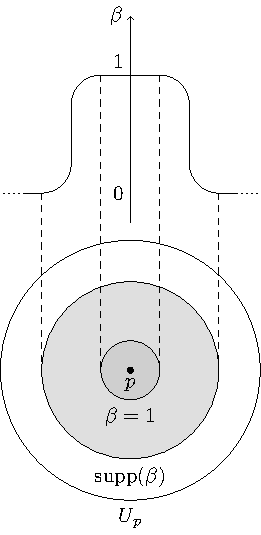
\includegraphics{riemann-ineq/figure}
	\caption{Constructing the smooth cutoff function $ \beta $.}
\end{marginfigure}

\begin{lemma}\label{lem:riemann-existence}
	$ \hat{\mathbb{C}} $ admits a non-constant meromorphic function.
	\begin{proof}
		Let us consider a single point $ p \in \hat{\mathbb{C}} $. We aim to
		construct a meromorphic function on $ \hat{\mathbb{C}} $ which has a simple
		pole at $ p $. In order to do this, consider the chart domain $ U_p $
		containing $ p $, and let $ z $ be a local coordinate in this chart. In this
		chart domain, $ 1/z $ is a meromorphic function, and we can extend this
		globally by introducing a \defined{cutoff function} $ \beta $. We define $
			\beta $ such that $ \supp ( \beta )\subset U_p $, and equal to $ 1 $ near $
			p$.

		The product $ \beta/z $ can be regarded as a function over $ X $; extending
		by zero outside of $ U_p $. Hence, the problem of finding a meromorphic
		function with a simple pole at $ p $ is equivalent to finding a function $ g
			\in \Omega^0(X) $ such that $ g+\beta/z \in \mathcal{O}( X \setminus \{ p \}
			) $.

		By Proposition~\ref{prop:hol} we know that this is equivalent to,
		\begin{align*}
			\overline{\partial }\left( g + \beta \cdot \frac{1}{z} \right)=0 \iff
			\overline{\partial }g = - \overline{\partial }\left( \beta \cdot \frac{1}{z}
			\right).
		\end{align*}

		A further application of Proposition~\ref{prop:hol}, and relabelling $ A =
			\overline{\partial }( \beta )1/z $, gives the simplification,
		\begin{align*}
			\overline{\partial }g = -A.
		\end{align*}
		If we consider the corresponding class $ [ A ]\in H ^{0,1}(X) $, we can see
		that the existence of a smooth function $ g $, is equivalent to the
		condition that $ A \in \im ( \overline{\partial } ) $, which is in turn
		equivalent to $ [ A ] = [ 0 ]\in H ^{0,1}(X) $. Our work in the previous
		section allows us to state that $ \dim H ^{0,1}(X)=0 $, which is enough to
		guarantee the existence of the function $ g $.
	\end{proof}
\end{lemma}

This is the most basic case in the proof of the following theorem. While we will
not provide a proof, it is intuitively clear how to proceed given a Riemann
surface of higher genus; adding sufficiently many poles, or in particular
sufficiently increasing $ \deg(D) $, forces a linear dependence between the
elements of the $ H ^{0,1}(X) $, which allows for the construction of the
promised meromorphic function.

\begin{theorem}[Riemann--Roch inequality]
	For a compact Riemann surface $ X $ of genus $ g $, and a divisor $ D $,
	\begin{align*}
		\dim L(D) \geq \deg(D) + 1 - g.
	\end{align*}
\end{theorem}

\begin{corollary}
	Every compact Riemann surface has a non-constant meromorphic function.
	\begin{proof}
		This follows directly from Riemann's inequality. If we take $ \deg(D) >g $,
		then
		\begin{align*}
			\dim L(D) \geq \deg(D) + 1 - g > g + 1 - g = 1,
		\end{align*}
		and hence there must be a non-constant function in $ L(D) $.
	\end{proof}
\end{corollary}

\begin{corollary}
	If $ X $ is a compact Riemann surface of genus $ 0 $, then $ X \cong
		\hat{\mathbb{C}} $.
	\begin{proof}
		If we take $ \deg(D)=1 $,
		\begin{align*}
			\dim L(D) \geq \deg(D)+1-g = 2,
		\end{align*}
		and in particular, there exists a meromorphic function which has a single,
		simple pole. Let $ p $ be this point, let $ \varphi:X \to \mathbb{C} $ be
		this function, and $ \Phi:X \to \hat{\mathbb{C}} $ the corresponding
		holomorphic representation. Then $ \deg(\Phi) = \deg(\Phi;\infty) =
			\mult(\Phi;p)=1 $, and hence $ \Phi $ is bijective, and further to this, a
		biholomorphism.
	\end{proof}
\end{corollary}

As mentioned previously, it was Gustav Roch, a student of Riemann, who
strengthened the inequality to an equality by incorporating the space of
meromorphic $ 1 $-forms associated to a canonical divisor. We will prove the first
case of the theorem, that is in the case where $ D $ is a non-negative divisor,
following Donaldson\sidenote{\footnotesize\cite[p. 115]{donaldson}}. We need a
final definition to prove the theorem in this restricted form.

\begin{definition}[Tangent residue]
	Let $ p \in X $ for a compact Riemann surface $ X $. Let $ f $ have a local
	Laurent series expansion about the point $ p $ as,
	\begin{align*}
		f = \sum_{i=-1}^{\infty}{a_{i}z^{i}}
	\end{align*}
	where $ z $ is the local coordinate centred at $ p $. Then, the
	\defined{tangent residue} of $ f $ is $ a_{-1}\frac{\partial }{\partial z} \in
		TX_{p} $ where $ TX_{p} $ denotes the tangent space at $ p $.
\end{definition}

\begin{marginfigure}
	\centering
	\resizebox{\columnwidth}{!}{
		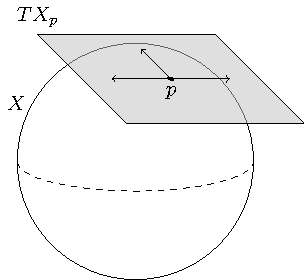
\includegraphics{tangent-space/figure}
	}
	\caption{A visualisation of $ T \hat{\mathbb{C}}_{p} $.}
\end{marginfigure}

\begin{theorem}[Riemann--Roch theorem]
	Let $ X $ be a compact Riemann surface, and $ K $ a canonical divisor on $ X $.
	Then, for any divisor $ D $,
	\begin{align*}
		\dim L(D) - \dim L(K-D) = \deg(D) + 1 - g.
	\end{align*}
	\begin{proof}
		As stated above, we will consider the case where $ D = p_{1}+ \cdots + p_{d}
		$ for $ p_{i} $ distinct points of $ X $. In this case, $ L(D) $ is the
		space of meromorphic functions which have at worst simple poles at each of
		the $ p_{i} $. Furthermore, the space $ L(K-D) $ can be recognised as the
		space of holomorphic $ 1 $-forms which vanish at each of the $ p_{i} $. This
		is understood by considering the fact that $ \omega \in L ( K-D ) \implies (
			\omega ) \geq D $, which imposes that $ \ord ( \omega;p_{i} ) \geq 1 $ for
		each $ 1 \leq i \leq d $.

		We aim to build the proof in stages, in an argument which relies heavily on
		results from linear algebra. Firstly, consider the inclusion defined as
		\begin{align*}
			I:\mathbb{C}\to L ( D ):c \mapsto f_{c} & : \mathbb{C}\to \mathbb{C} \\
			                                        & : z \mapsto c,
		\end{align*}
		i.e., a map which takes the constants in $ \mathbb{C} $ to their respective
		constant maps $ f_{c} $. We can make initial note of the fact that the image
		of $ I $, $ \im I $, is the set of complex valued constant functions.

		We consider also the map
		\begin{align*}
			R: L(D) \to \bigoplus_{i=1}^{d}{TX_{p_{i}}},
		\end{align*}
		which maps the meromorphic function $ f $ to its tangent residues in the
		local coordinates $ z_{i} $ of each of the $ p_{i} $. The kernel of the map,
		is the collection of functions which have zero residue at every one of the
		$ p_{i} $, and since we are considering the case of $ D(p) \in \{ 0,1 \} $,
		this is exactly the set of holomorphic functions. Furthermore, we know that
		holomorphic functions are constant, and therefore, $ \ker R = \im I $. In
		particular, we have an exact sequence of vector spaces,
		\begin{align*}
			\mathbb{C}\xrightarrow{\ I\ } L(D)\xrightarrow{\ R\ }
			\bigoplus_{i=1}^{d}{TX_{p_{i}}}.
		\end{align*}
		We can relate the dimensions of these spaces using the rank nullity theorem,
		\begin{align*}
			\dim L(D) & = \dim\im R + \dim\ker R \\
			          & = \dim\im R + \dim\ker I \\
			          & = \dim\im R + 1,
		\end{align*}
		hence our interest now lies in the space $ \im R $.

		In the same vein as our previous work, we aim to find a map whose kernel is
		the same as $ \im R $. With this in mind, we consider the family of maps
		\begin{align*}
			A_{i}:TX_{p_{i}} \to H^{0,1}(X),
		\end{align*}
		which for a local coordinate $ z_{i} $ centered on $ p_{i} $, maps $
			\partial/\partial z_{i} $ to the cohomology class $ [ A_{i} ] $ where $
			A_{i} $ is defined in the same way as in the proof of
		Lemma~\ref{lem:riemann-existence}, that is, as the global extension of $
			\overline{\partial}( \beta_{i} \cdot 1/z_{i} ) $. We therefore have a map
		\begin{align*}
			\underline{A}: \bigoplus_{i=1}^{d}{TX_{p_{i}}} \to H^{0,1}(X):
			( t_{1},...,t_{d} )\mapsto \sum_{i=1}^{d}{A_{i}( t_{i} )}.
		\end{align*}
		and aim to show that $ \im R = \ker \underline{A} $. To begin, consider
		an element $ R ( f ) = ( \lambda_{1}\cdot \partial/\partial z_{1},...,
			\lambda_{d}\cdot \partial/\partial z_{d} ) $, and the map
		\begin{align*}
			F = f - \sum_{i=1}^{d}{\lambda_{i}\beta_{i}\frac{1}{z_{i}}},
		\end{align*}
		which is, by design a smooth function on $ X $. Therefore, $ [
					\overline{\partial }F ]=0 $ in $ H^{0,1}(X) $, and furthermore, since $ f $
		is holomorphic away from the points $ p_{i} $, $ \overline{\partial }f=0 $
		away from these points, and a natural extension to $ 0 $ over these points
		gives,
		\begin{align*}
			\left[\overline{\partial }\left(
			\sum_{i=1}^{d}{\lambda_{i}\beta_{i}\frac{1}{z_{i}}} \right) \right] & =
			[\overline{\partial }f ]                                                   \\
			\left[\overline{\partial }\left(
			\sum_{i=1}^{d}{\lambda_{i}\beta_{i}\frac{1}{z_{i}}} \right) \right] & = 0  \\
			\sum_{i=1}^{d}{\lambda_{i}[ A_{i} ]}                                & = 0,
		\end{align*}
		and in particular, $ \im R \subseteq \ker \underline{A} $. To show the other
		inclusion, consider $ \underline{\alpha} = ( \alpha_{1}\partial/\partial
			z_{1},..., \alpha_{d}\partial/\partial z_{d} )\in \ker \underline{A} $. By
		the definition of $ \underline{A} $, this is equivalent to
		\begin{align*}
			\underline{A}( \underline{\alpha} ) = 0 \in H^{0,1}(X),
		\end{align*}
		which is equivalent to the existence of a function $ g \in \Omega^{0}(X) $
		such that,
		\begin{align*}
			\overline{\partial }g = - \underline{A}( \underline{\alpha} ).
		\end{align*}
		Rearranging this expression gives us that
		\begin{align*}
			\overline{\partial }\underbrace{\left( g+
				\alpha_{1}\beta_{1}\frac{1}{z_{1}}+ \cdots +
				\alpha_{d}\beta_{d}\frac{1}{z_{d}} \right)}_{G \in L(D)}=0,
		\end{align*}
		and since $ R(G)=\underline{\alpha} $, $ \ker \underline{A}\subseteq \im R
		$, and in particular $ \im R = \ker \underline{A} $.

		Hence we can extend our exact sequence,
		\begin{align*}
			\mathbb{C}\xrightarrow{\ I\ } L(D)\xrightarrow{\ R\ }
			\bigoplus_{i=1}^{d}{TX_{p_{i}}}\xrightarrow{\ \underline{A}\ } H^{0,1}(X),
		\end{align*}
		and rephrase our previous expression as,
		\begin{align*}
			\dim L(D) & = \dim\ker \underline{A} + 1.
		\end{align*}

		In order to compute $ \dim\ker \underline{A} $, we consider the transpose of
		this map,
		\begin{align*}
			\underline{A}^{T}: \left( H^{0,1}(X) \right)^{*}\to \left(
			\bigoplus_{i=1}^{d}{TX_{p_{i}}} \right)^{*} = \bigoplus_{i=1}^{d}{T
				^{*}X_{p_{i}}},
		\end{align*}
		and use elementary linear algebraic relations, together with the fact that $
			\dim H^{0,1}(X)=g $,
		\begin{align*}
			\dim\bigoplus{TX_{p_{i}}} - \dim H^{0,1}(X) & = \dim\im \underline{A} +
			\dim\ker \underline{A}
			\\ & \quad - \dim\im
			\underline{A}^{T} - \dim\ker
			\underline{A}^{T}
			\\ \deg(D)-g
			                                            & = \dim\ker \underline{A} -
			\dim\ker \underline{A}^{T}.
		\end{align*}

		From Corollary~\ref{cor:dual-space-iso} we know that $ ( H^{0,1}(X)
			)^{*}\cong H^{1,0}(X) $ and consequently, we define a final map
		\begin{align*}
			E:H^{1,0}\to \bigoplus_{i=1}^{d}{T ^{*}X_{p_{i}}}:\omega \mapsto (
			\omega ( p_{1} ),..., \omega ( p_{d} ) ).
		\end{align*}

		It can be shown\sidenotemark\ that $ \underline{A}^{T} = 2 \pi i E $, and
		noticing that $ \ker E$ is the space of holomorphic $ 1 $-forms which vanish
		at every point $ p_{i} $ gives,
		\begin{align*}
			\dim L(D)                              & = 1 + \dim\ker \underline{A} \\
			\dim L(D) - \dim\ker \underline{A}^{T} & = 1 + \deg(D) - g            \\
			\dim L(D) - \dim\ker E                 & = 1 + \deg(D) - g            \\
			\dim L(D) - \dim L(K-D)                & = 1 + \deg(D) - g.
		\end{align*}
	\end{proof}
\end{theorem}
\sidenotetext[][-10\baselineskip]{\footnotesize\cite[p. 116]{donaldson}}

\chapter*{Conclusion}
With the proof of the Riemann--Roch theorem in its restricted form comes the end
of this report. Discussion of the full proof of the theorem would involve some
preliminary work with sheaf theory, and unfortunately, any attempt to introduce
the necessary constructions would be either rushed or incomplete. A full
treatment of the Riemann--Roch theorem can be found in
Forster\sidenote{\footnotesize\cite{forster}}, and there are clear similarities
between this proof and the one which we have presented.

A natural next step in the study of Riemann surfaces would be to explore the
Uniformisation theorem, which is a result aimed at the classification of the
simply connected Riemann surfaces, conjectured in 1882 by Felix Klein ``in the
midst of an asthma attack''\sidenote{\footnotesize\cite{abikoff}}.

\begin{theorem}[Uniformisation Theorem]
	Every simply connected Riemann surface is biholomorphic to one of $ \mathbb{C}
	$, $ \hat{\mathbb{C}} $, or the unit disc $ \mathbb{D} $.
\end{theorem}

\begin{figure*}
	\centering
	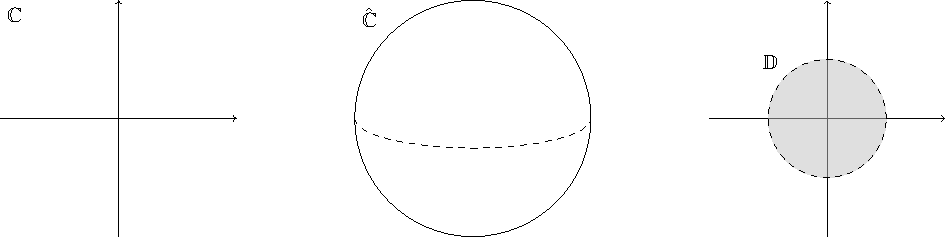
\includegraphics{uniformisation/figure}
	\caption{Drawing every simply connected Riemann surface.}
\end{figure*}

Donaldson\sidenote{\footnotesize\cite[Ch. 10]{donaldson}} explores this result
in full detail, and the proof ultimately hinges on an analogue of the main
analytic result of this report, Theorem~\ref{thm:main-thm}.

There are some further reaching consequences of the existence of meromorphic
functions which we did not explore. The most famous of these consequences was
proved by Riemann, and was the initial motivation for his pursuit of a bound on
the number of linearly independent meromorphic functions. Riemann proved that
all compact Riemann surfaces can be embedded in projective space, and hence the
study of compact Riemann surfaces can be rephrased as the study of one
dimensional projective varieties.

This duality in the theory of projective geometry and analytic manifold theory
is extended in higher dimensions, and one may consider further exploration in
the direction of closely related concepts such as Riemannian manifolds, and
further to this K\"ahler manifolds. In fact, fixing some metric on the Riemann
surface gives some element of simplification to the arguments presented in
Chapter~\ref{ch:poisson-eq}, and many of the results presented admit logical
generalisations.

% {\it
% 	It is with a heavy hand that I write the final words of this report, with
% 	tired eyes that I read it for the final time. The beauty and depth of this area
% 	of mathematics has been captivating, and I can only hope to have adequately
% 	portrayed this.
% }


\newgeometry{inner=2cm, outer=2cm, top=2cm, bottom=2cm}
\printindex
\printbibliography[heading=bibintoc]
\end{document}
